% !TEX program = xelatex
%%%%%%%%%%%%%%%%%%%%%%%%

\documentclass[11pt,aspectratio=169]{beamer} % 11pt is default
\usetheme{metropolis} % [progressbar=frametitle]
\setbeamercolor{background canvas}{bg=white}
\setbeamertemplate{caption}{\insertcaption} 
\setbeamersize{text margin left=2em,text margin right=2em}
\setbeamertemplate{frame footer}{\vspace{-5pt}}

\usepackage[round]{natbib}
\usepackage{amsmath}
\usepackage{mathtools}
\usepackage[group-minimum-digits=4,group-separator={,}]{siunitx}
\usepackage{graphicx}
\usepackage{wrapfig}
\usepackage{multimedia}

\usepackage{tikz}
\usetikzlibrary{backgrounds}
\usetikzlibrary{arrows,shapes}
\usetikzlibrary{tikzmark}
\usetikzlibrary{calc}
\usepackage[dvipsnames]{xcolor}

\usepackage[skins,theorems]{tcolorbox}
\usepackage{pdfpages}
\usepackage{colortbl}
\usepackage{changepage}
\usepackage{booktabs}
\usepackage{makecell}
\usepackage{setspace}
\usepackage{algorithm}
\usepackage[noend]{algpseudocode}
\usepackage{subcaption}
\usepackage[framemethod=TikZ]{mdframed}
\usepackage{xspace}

\usepackage{annotate-equations}

% Shortcut for beamer frames
\newcommand{\bframe}[2][c]{\begin{frame}[#1]{#2}}
\newcommand{\eframe}{\end{frame}} % \eframe causes problems for some reason

% Shortcut for bold text
\newcommand{\fat}[1]{\textbf{#1}}

% Boxing items on slide
\newcommand{\Cboxed}[2]{\colorlet{currentcolor}{.}{\color{#1}\fbox{\color{currentcolor}#2}}} %create coloured box around equation

% checkmark and xmark
\usepackage{pifont}
\newcommand{\cmark}{\ding{51}}%
\newcommand{\xmark}{\ding{55}}%

% Highlighting text in orange
\newcommand{\e}[1]{\alert{#1}}

% Underline
\newcommand{\uline}[1]{\underline{#1}}

% Include figure
\newcommand{\imgw}[2]{\includegraphics[width=#2\textwidth]{#1}} % \imgw{file}{height-scale}
\newcommand{\imgh}[2]{\includegraphics[height=#2\textheight]{#1}} % \imgh{file}{width-scale}

% Shortcut for latex commands
\newcommand{\blist}{\vspace{-3pt}\begin{list}{\raisebox{1pt}{\small$\bullet$}}{\leftmargin=13pt\itemsep=4pt}}
\newcommand{\blisttab}{\vspace{5pt}\blist}
\newcommand{\elisttab}{\end{list}}
\newcommand{\listtab}{\\[3pt] $\Rightarrow$ }
\newcommand{\elist}{\end{list}\vspace{5pt}}
\newcommand{\bblock}[1]{\metroset{block=fill}\begin{block}{#1}}
\newcommand{\eblock}{\end{block}}
\newcommand{\bmath}[1][0]{\begin{equation*}\hspace{#1em}}
\newcommand{\emath}{\end{equation*}}
\newcommand{\bcol}{\begin{columns}}
\newcommand{\col}[1]{\column{#1\textwidth}}
\newcommand{\tcol}[1]{\column[T]{#1\textwidth}}
\newcommand{\ecol}{\end{columns}}
\newcommand{\place}[4]{\begin{textblock}{#3}(#1,#2) #4 \end{textblock}} % \place{x}{y}{width}{text}
\newcommand{\placeframed}[4]{\place{#1}{#2}{#3}{\fbox{\parbox{#3em}{#4}}}}
\newcommand{\placeimg}[4]{\place{#1}{#2}{#3}{\imgw{#4}{1}}} % \placeimg{x}{y}{width}{file}
\newcommand{\videolink}[2]{\movie[externalviewer]{{\bf Video:} #1}{videos/#2}} % \videolink{title}{file}
\newcommand{\btab}[1]{\begin{tabular}{#1}}
\newcommand{\etab}{\end{tabular}}
\newcommand{\balgo}[2][1.3]{{#2:} \\[5pt] \begin{algorithmic}[1] \linespread{#1}\selectfont}
\newcommand{\ealgo}{\end{algorithmic}}
\renewcommand{\algorithmicloop}{\textbf{repeat:}}
\newcommand{\cred}{\cellcolor{red!25}}
\newcommand{\cgreen}{\cellcolor{green!25}}

% Shortcut for commonly used math symbols
\newcommand{\condpr}[2]{\text{Pr}\hspace{-1pt}\left\{ #1 \ \mid \ #2 \right\}}
\newcommand{\exarg}[2]{\mathbb{E}_{#1}\hspace{-2pt}\left[ #2 \right]}
\newcommand{\exnoarg}[1]{\mathbb{E}_{#1}}
\NewDocumentCommand\ex{ m g }{
	\IfNoValueTF{#2}{\exnoarg{#1}}{\exarg{#1}{#2}}
}
\newcommand{\der}[2]{\frac{\partial #1}{\partial #2}}
\newcommand{\stats}{\mathcal{S}}
\newcommand{\acts}{\mathcal{A}}
\newcommand{\rews}{\mathcal{R}}
\newcommand{\eps}{\mathcal{E}}
\newcommand{\ver}{\,\vert\,}
\newcommand{\vhat}{\hat{v}}
\newcommand{\qhat}{\hat{q}}
% \newcommand{\para}{\textbf{w}}
\newcommand{\feats}{\textbf{x}}
\newcommand{\elig}{\textbf{z}}
\newcommand{\gradient}{\nabla}
\newcommand{\outline}{Lecture Outline}
\newcommand{\reading}{Reading}
\newcommand{\h}[1]{\emph{#1}}

\emph
% \newcommand{\lindex}[1]{%
% 	\lowercase{\def\temp{#1}%
% 	\expandafter\index\expandafter{\temp}%
% }

\newcommand{\indx}[1]{\index{#1}}
\newcommand{\hind}[1]{\h{#1}\lindex{#1}}

% Set of real numbers
\newcommand{\R}{\mathbb{R}}
% Proportional to
% Transpose of a vector x
\newcommand{\vectranspose}[1]{#1^\top}
% Transpose of a matrix X
\newcommand{\mattranspose}[1]{#1^\top}
% Probability
\newcommand{\pr}{\text{Pr}}
% Conditional probability of x given y
\newcommand{\cpr}[2]{\pr( #1 \mid #2 )}
% x sampled according to probability distribution p
\newcommand{\sampled}[2]{#1 \sim #2}
% Assign value y to variable x
\newcommand{\assign}[2]{#1 \gets #2}
% Training data set
\newcommand{\data}{\mathcal{D}}
% Concatenation of inputs a, b, c, ...
\newcommand{\con}[1]{\langle #1 \rangle}
% array with bracket
\newcommand{\bra}[2]{\left[ \begin{array}{#1} #2 \end{array} \right]}
% Indicator function: returns 1 if x is true, otherwise returns 0
\newcommand{\ind}[1]{[#1]_1}

% common way of referring to places
\newcommand{\seehere}[1]{(\cref{#1})}

% shortcut text commands
\newcommand{\rl}{RL\xspace}
\newcommand{\marl}{MARL\xspace}
\newcommand{\ctde}{CTDE\xspace}
\newcommand{\sa}{single-agent\xspace}
\newcommand{\ma}{multi-agent\xspace}
\newcommand{\Ma}{Multi-agent\xspace}
\newcommand{\mas}{multi-agent system\xspace}
\newcommand{\stat}{stationarity\xspace}
\newcommand{\nonstat}{non-stationarity\xspace}
\newcommand{\pg}{policy gradient\xspace}
\newcommand{\vb}{value-based\xspace}
\newcommand{\pbt}{population-based training\xspace}
\newcommand{\psro}{policy space response oracles\xspace}
\newcommand{\Psro}{Policy space response oracles\xspace}
\newcommand{\sct}{\emph{StarCraft~II}\xspace}
\newcommand{\as}{AlphaStar\xspace}
\newcommand{\az}{AlphaZero\xspace}
\newcommand{\lbf}{level-based foraging\xspace}
\newcommand{\Lbf}{Level-based foraging\xspace}
\newcommand{\nfg}{normal-form game\xspace}
\newcommand{\nfgs}{normal-form games\xspace}
\newcommand{\Nfg}{Normal-form game\xspace}
\newcommand{\Nfgs}{Normal-form games\xspace}
\newcommand{\rps}{Rock-Paper-Scissors\xspace}
\newcommand{\pd}{Prisoner's Dilemma\xspace}
\newcommand{\survey}[4]{\noindent #1 (#4). ``#2.'' In: {\it #3}. \\}
\newcommand{\nashprob}{\textsc{Nash}\xspace}
\newcommand{\eol}{\textsc{End-of-Line}\xspace}
\newcommand{\ul}[1]{\underline{#1}}
\newcommand\norm[1]{\lVert#1\rVert}
\newcommand{\qlearn}{Q-learning\xspace}
\newcommand{\sarsa}{Sarsa\xspace}
\newcommand{\bayes}{Bayesian\xspace}
\newcommand{\bellman}{Bellman\xspace}
\newcommand{\markov}{Markov\xspace}
\newcommand{\pareto}{Pareto\xspace}
\newcommand{\boltzmann}{Boltzmann\xspace}
\newcommand{\mc}{Monte Carlo\xspace}
\newcommand{\nash}{Nash\xspace}
\newcommand{\ppad}{PPAD}
\newcommand{\dqn}{deep Q-networks\xspace}
\newcommand{\reinforce}{REINFORCE\xspace}
\newcommand{\qmix}{QMIX\xspace}
\newcommand{\qtran}{QTRAN\xspace}
\newcommand{\adam}{Adam\xspace}
\newcommand{\nret}{{$N$}-step returns\xspace}

% COMMANDS FOR COMMON NOTATION

% agent set
% state space
\newcommand{\St}{S}
\newcommand{\Stterm}{\bar{\St}}
% state
\newcommand{\st}{s}
\newcommand{\sth}{\hat{\st}}
% observation space
\newcommand{\Ob}{O}

% observation
\newcommand{\ob}{o}

% joint observation
\newcommand{\job}{o}
% action space
\newcommand{\Ac}{A}

% action
\newcommand{\ac}{a}
\newcommand{\ach}{\hat{\ac}}

% joint action
\newcommand{\jac}{a}
% reward
\newcommand{\rew}{r}
\newcommand{\rewh}{\hat{\rew}}
% centralised information
\newcommand{\ci}{z}

% initial state distribution

\newcommand{\instdist}{\mu}
% % state transition function

\newcommand{\Stf}{\mathcal{T}}
% % simulation/sampling model
\newcommand{\Stfsim}{\widehat{\Stf}}

% observation function
\newcommand{\Obf}{\mathcal{O}}

% reward function
\newcommand{\Rew}{\mathcal{R}}

% POLICIES, RETURNS, VALUES

% policy space
\newcommand{\Pol}{\Pi}

% policy
\newcommand{\pol}{\pi}
\newcommand{\poltil}{\tilde{\pol}}

% set of histories
\newcommand{\His}{H}
\newcommand{\Fhis}{\hat{\His}}
% history
\newcommand{\his}{h}

% full history
\newcommand{\fhis}{\hat{\his}}

% observation history extracted from full history
\newcommand{\obsext}{\sigma}

% discount factor
\newcommand{\dsc}{\gamma}

% return
\newcommand{\ret}{u}

% expected return for joint policy
\newcommand{\exret}{U}

% Agents
\newcommand{\Ag}{I}

% RL / MARL

% learning algorithm

\newcommand{\alg}{\mathbb{L}}

% empirical distribution/ average policy
\newcommand{\empdis}{\bar{\pol}}
\newcommand{\avgpol}{\bar{\pol}}
\newcommand{\agmod}{\hat{\pol}}
\newcommand{\Agmod}{\hat{\Pol}}
\newcommand{\agmodj}{agent model for agent $j$}

% best response
\newcommand{\br}{\textnormal{BR}}

% game value
\newcommand{\gval}{Value}

% value under agent model
\newcommand{\amval}{AV}

% regret
\newcommand{\regret}{Regret}
\newcommand{\avgreg}{\bar{R}}
% TD target
\newcommand{\target}{\mathcal{X}}
% step size (for gradient-based MARL in Chapter 5)
\newcommand{\step}{\kappa}


% DEEP LEARNING

% parameters
\newcommand{\para}{\theta}

% loss
\newcommand{\loss}{\mathcal{L}}
% batch
\newcommand{\batch}{\mathcal{B}}
\newcommand{\batchsize}{B}

% etnropy
\newcommand{\entropy}{\mathcal{H}}

% Create algorithm environment
\newcommand{\balg}[2]{
  \begin{algorithm}[H]
    \caption{#1}
    \label{alg:#2}
    \setstretch{1.1}
    \begin{algorithmic}[1]}

\newcommand{\ealg}{
    \end{algorithmic}
  \end{algorithm}}

% Argmin/ Argmax operators

\DeclareMathOperator*{\argmin}{arg\,min} 
\DeclareMathOperator*{\argmax}{arg\,max}

\makeatletter
\newenvironment{myitemize}{%
   \setlength{\topsep}{0pt}
   \setlength{\partopsep}{0pt}
   \renewcommand*{\@listi}{\leftmargin\leftmargini \parsep\z@ \topsep\z@ \itemsep\z@}
   \let\@listI\@listi
   \itemize
}{\enditemize}
\makeatother  

% define widebar for target parameters
\makeatletter
\newcommand*\rel@kern[1]{\kern#1\dimexpr\macc@kerna}
\newcommand*\widebar[1]{%
	\begingroup
	\def\mathaccent##1##2{%
		\rel@kern{0.8}%
		\overline{\rel@kern{-0.8}\macc@nucleus\rel@kern{0.2}}%
		\rel@kern{-0.2}%
	}%
	\macc@depth\@ne
	\let\math@bgroup\@empty \let\math@egroup\macc@set@skewchar
	\mathsurround\z@ \frozen@everymath{\mathgroup\macc@group\relax}%
	\macc@set@skewchar\relax
	\let\mathaccentV\macc@nested@a
	\macc@nested@a\relax111{#1}%
	\endgroup
}
\makeatother


% MATRIX GAMES

\newcolumntype{?}{!{\vrule width 1pt}}
\newcommand{\bhline}{\Xhline{1pt}}
\newcommand{\gametwo}[3]{
	\begin{tabular}{c?c|c}
		 & #1 \\
		\bhline
		#2    \\
		\hline
		#3    \\
	\end{tabular}
}
\newcommand{\gamethree}[4]{
	\begin{tabular}{c?c|c|c}
		 & #1 \\
		\bhline
		#2    \\
		\hline
		#3    \\
		\hline
		#4    \\
	\end{tabular}
}

\newcommand{\gamepd}{
    % \gametwo{C & D}{C & -1,-1 & -5,0}{D & 0,-5 & -3,-3}
	\begin{tabular}{c|c|c}
	& C & D \\
	\hline
	C & -1,-1 & -5,0 \\
	\hline
	D & 0,-5 & -3,-3
	\end{tabular}
}

\newcommand{\gamerps}{
    % \gamethree{R & P & S}{R & 0,0 & -1,1 & 1,-1}{P & 1,-1 & 0,0 & -1,1}{S & -1,1 & 1,-1 & 0,0}
	\begin{tabular}{c|c|c|c}
	& R & P & S \\
	\hline
	R & 0,0 & -1,1 & 1,-1 \\
	\hline
	P & 1,-1 & 0,0 & -1,1 \\
	\hline
	S & -1,1 & 1,-1 & 0,0
	\end{tabular}
}

\newcommand{\gamecoord}{
    % \gametwo{A & B}{A & 10 & 0}{B & 0 & 10}
	\begin{tabular}{c|c|c}
		& A & B \\
		\hline
		A & 10 & 0 \\
		\hline
		B & 0 & 10 \\
	\end{tabular}
}

\newcommand{\gamechicken}{
    % \gametwo{S & L}{S & 0,0 & 7,2}{L & 2,7 & 6,6}
	\begin{tabular}{c|c|c}
		& S & L \\
		\hline
		S & 0,0 & 7,2 \\
		\hline
		L & 2,7 & 6,6
	\end{tabular}
}

\newcommand{\gamestaghunt}{
    % \gametwo{S & H}{S & 4,4 & 0,3}{H & 3,0 & 2,2}
	\begin{tabular}{c|c|c}
		& S & H \\
		\hline
		S & 4,4 & 0,3 \\
		\hline
		H & 3,0 & 2,2
	\end{tabular}
}

\newcommand{\gamebattle}{
    \begin{tabular}{c|c|c}
    & A & B \\
    \hline
    A & 10,7 & 2,2 \\
    \hline
    B & 0,0 & 7,10
    \end{tabular}
}

\newcommand{\gameepsne}{
    % \gametwo{C & D}{A & 100,100 & 0,0}{B & 1,2 & 1,1}
	\begin{tabular}{c|c|c}
		& C & D \\
		\hline
		A & 100,100 & 0,0 \\
		\hline
		B & 1,2 & 1,1
	\end{tabular}
}

% Define colorboxes
\tcbset{
  % Defaults
  my box/main style/.style={},
  my box/title style/.style={},
  % Use the 'append' variants if you want to add to the defaults instead of
  % overriding them.
  my box/main/.style={/tcb/my box/main style/.style={#1}},
  my box/title/.style={/tcb/my box/title style/.style={#1}},
  my box/append main/.style={/tcb/my box/main style/.append style={#1}},
  my box/append title/.style={/tcb/my box/title style/.append style={#1}},
  %
  my box/.style={
    my box/.cd, #1,
    /tcb/.cd,
    enhanced,
    my box/main style,
    attach boxed title to top left={xshift=0.2cm, yshift=-0.2cm},
    top=10pt,
    boxed title style={
      outer arc=0pt,
      arc=0pt,
      top=3pt,
      bottom=3pt,
      my box/title style,
    },
  },
}

% define 'solutionbox' environment with coloured box
\newtcolorbox{solutionbox}[1][]{
  my box={
    main={colframe=green!40!gray!90, colback=green!20!gray!5},
    title={colback=green!40!gray!90},
  },
  title=Solution,
  #1,
}

\newtcolorbox{problembox}[1][]{
  my box={
    main={colframe=red!40!gray!90, colback=red!20!gray!5},
    title={colback=red!40!gray!90},
  },
  title=Problem,
  #1,
}

\newtcolorbox{notebox}[1][]{
  my box={
    main={colframe=orange!40!gray!80, colback=orange!20!gray!5},
    title={colback=orange!40!gray!80},
  },
  title=Note,
  #1,
}

\newtcolorbox{intuitionbox}[1][]{
  my box={
    main={colframe=blue!60!gray!80, colback=blue!20!gray!5},
    title={colback=blue!60!gray!80},
  },
  title=Intuition,
  #1,
}

\newtcolorbox{reminderbox}[1][]{
  my box={
    main={colframe=black!40!gray, colback=gray!10!white},
    title={colback=black!40!gray},
  },
  title=Reminder,
  #1,
}

\newtcolorbox{custombox}[2][]{
  my box={
    main={colframe=black!40!gray, colback=gray!10!white},
    title={colback=black!40!gray},
  },
  title={#2},
  #1,
}

% no title boxes
\newtcolorbox{greenbox}[1][]{
  my box={
    main={colframe=green!40!gray!90, colback=green!20!gray!5},
  },
  #1,
}
\newtcolorbox{redbox}[1][]{
  my box={
    main={colframe=red!40!gray!90, colback=red!20!gray!5},
  },
  #1,
}
\newtcolorbox{orangebox}[1][]{
  my box={
    main={colframe=orange!40!gray!80, colback=orange!20!gray!5},
  },
  #1,
}
\newtcolorbox{bluebox}[1][]{
  my box={
    main={colframe=blue!60!gray!80, colback=blue!20!gray!5},
  },
  #1,
}
\newtcolorbox{blackbox}[1][]{
  my box={
    main={colframe=black!55!black, colback=gray!5!white},
  },
  #1,
}


% Define intro slide command
\newcommand{\introslide}{
    \begin{frame}{MARL Book}
        \begin{columns}
            \begin{column}{0.5\textwidth}
            \begin{figure}
              \centering
              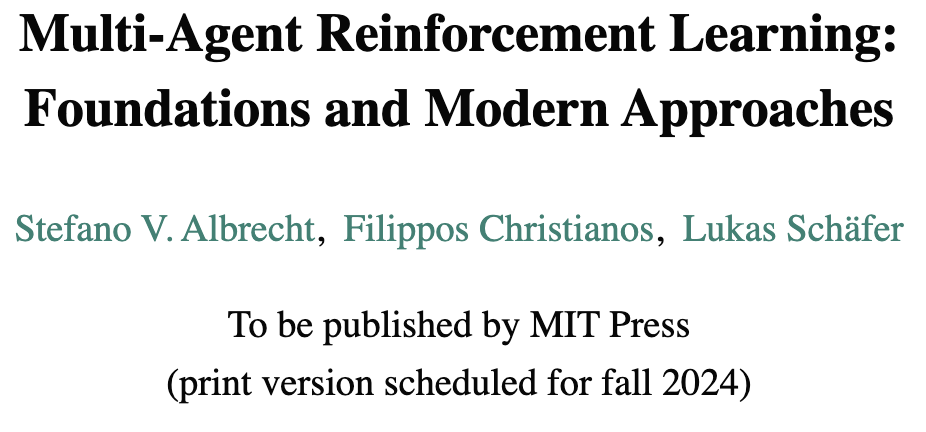
\includegraphics[width=\textwidth,height=.8\textheight,keepaspectratio]{images/1_MARL_book.png}
            
              \label{fig:enter-label}
            \end{figure}
          \end{column}
        
        \hspace{20pt}
            
          % Column for the text
            \begin{column}{0.45\textwidth}
	        \small

                This lecture is based on \textit{Multi-Agent Reinforcement Learning: Foundations and Modern Approaches} by Stefano V. Albrecht, Filippos Christianos and Lukas Sch\"afer
                
                \vspace{20pt}
                
                The book can be downloaded for free at \textcolor{blue}{\href{https://www.marl-book.com/}{www.marl-book.com}}.
            \end{column}
        
        \end{columns}
    \end{frame}
}

\newcommand{\leoslide}{
  \author{Stefano V. Albrecht, Filippos Christianos, Lukas Sch\"afer \\ Slides by: Leonard Hinckeldey}
}

\newcommand{\otherslide}{
  \author{Stefano V. Albrecht, Filippos Christianos, Lukas Sch\"afer}
}
	
\title{Multi-Agent Reinforcement Learning}
\date{}

\hypersetup{
  pdfsubject = {Multi-Agent Reinforcement Learning},
}

\otherslide

\subtitle{Multi-Agent Deep Reinforcement Learning -- Part 2}

\begin{document}
\maketitle

\introslide

\begin{frame}{\outline}

\blist
    \item Agent modeling with deep learning
    \item Parameter and experience sharing
    \item Policy self-play in zero-sum games
    \item Population-based training
\elist
\end{frame}

\section{Agent Modeling with Deep Learning}

\begin{frame}[t]{Agents Modeling -- Motivation}
    In MARL, agents need to consider the policies of other agents to coordinate their actions.

    \pause

    Approaches presented so far account for the action selection of other agents through:
    \blist
        \item Distribution of training data is dependent on the policies of all agents
        \item Training centralized critics conditioned on the actions of other agents
    \elist

    \pause

    \begin{redbox}
        Can we provide agents with more \fat{explicit} information about the policies of other agents so they can learn to coordinate better, e.g.\ by learning best-response policies?
    \end{redbox}
\end{frame}

\begin{frame}[t]{Recap: Agent Modeling}
    \begin{reminderbox}
        In Chapter 6, we have seen approaches that model other agents' policies:

        \blist
            \item Learn models of other agents to predict their actions
            \item Compute optimal action (best-response) against agent models
        \elist

        \begin{center}
            \imgw{images/chapter6/agentmodel.pdf}{0.90} \\[1.5em]
        \end{center}

        S. Albrecht, P. Stone. {\bf Autonomous Agents Modelling Other Agents: A Comprehensive Survey and Open Problems.} {\it Artificial Intelligence}, 2018
    \end{reminderbox}
\end{frame}

\begin{frame}[t]{Recap: Tabular Agent Modeling}
    In Chapter 6, we modeled other agents' policies as stationary distributions by maintaining tables of action frequencies for each state

    \pause

    \begin{problembox}
        Similar to tabular value functions, \fat{tabular agent models} are limited due to their inability to generalise across states.
    \end{problembox}

    \pause

    \begin{solutionbox}
        Use \fat{deep learning} to learn generalisable agent models!
    \end{solutionbox}
\end{frame}

\begin{frame}[t]{Recap: Joint-Action Learning with Agent Models}
    \begin{reminderbox}
        We have already seen \e{joint-action learning with agent models} (JAL-AM)

        \blist
            \item<2-> Agents learn models of other agents $j$ conditioned on states $\st$: $\agmod_{-i}(\jac_{-i} \mid \st)$
            \item<3-> Agents learn value functions conditioned on the joint action: $Q_i(\st, \jac)$
            \item<4-> Using the value function and agent models, agent $i$ can compute its expected action values under the current models of other agents:
                \bmath
                    \amval_i(\st,\ac_i) = \sum_{\ac_{-i} \in \Ac_{-i}} Q_i(\st, \con{\ac_i,\ac_{-i}}) \prod_{j \in \Ag \setminus \{i\}} \agmod_j(\ac_j \mid \st)
                \emath
            \item<5-> Use $\amval_i$ to select optimal actions and as learning update targets
        \elist
    \end{reminderbox}
\end{frame}


\begin{frame}[t]{Joint-Action Learning with \fat{Deep} Agent Models}
    How to do this with deep learning for partially observable environments (POSG)?
    \blist
        \item<2-> Represent agent $i$'s model of agent $j$ as a neural network: $\agmod^i_{j}(\ac_{j} \mid \his_i; \phi^i_j)$
        \item<2-> Given the observation history of agent $i$, its model $\agmod^i_{j}(\ac_{j} \mid \his_i; \phi^i_j)$ for agent $j$ outputs a probability distribution over actions
        \item<3-> Agent $i$ can train its model for agent $j$ by minimizing the cross-entropy loss between the predicted policy $\agmod_j^i$ and the observed actions of agent $j$:
            \bmath
                \loss(\phi^i_j) = \ex{\ac_j^t \sim \pol_j(\his_j^t)}{- \log \agmod^i_j(\ac_j^t \mid \his_i^t; \phi^i_j)}
            \emath
        \item<4-> Then, agent $i$ can compute expected action values:
        \bmath
            AV(\his_i, \ac_i; \theta_i) = \sum_{\ac_{-i}\in\Ac_{-i}} Q(\his_i, \con{\ac_i, \ac_{-i}}; \theta_i) \prod_{j \neq i} \hat\pol_{j}^i(\ac_{j} \mid \his_i; \phi_j^i) 
        \emath
    \elist
\end{frame}

\begin{frame}[t]{Joint-Action Learning with \fat{Deep} Agent Models}

    \vspace{-1em}

    \begin{problembox}
        To compute $AV$, we need to sum over all possible joint actions of other agents which is infeasible for environments with large action spaces or many agents.
    \end{problembox}

    \pause

    \begin{solutionbox}
        Approximate $AV$ with only $K$ joint actions sampled from the agent models:
        \bmath
            AV(\his_i, \ac_i; \theta_i) = \frac{1}{K} \sum_{k=1}^K Q(\his_i, \con{\ac_i, \jac_{-i}^k}; \theta_i)\bigg\rvert_{\ac^k_j \sim \hat\pol_j^i(\cdot \mid \his_i)}
        \emath
    \end{solutionbox}

    \pause

    To optimise the centralized joint-action-value function of agent $i$, we then minimize the following loss over batches of experiences sampled from a replay buffer:
    \bmath
        \loss(\theta_i) = \frac{1}{\batchsize} \sum_{(\his_i^t, \ac^t, \rew_i^t, \his_i^{t+1}) \in \batch} \left(\rew_i^t + \dsc \max_{\ac_i'\in\Ac_i} AV(\his_i^{t+1}, \ac_i'; \widebar{\theta}_i) - Q(\his_i^t, \con{\ac_i^t, \jac_{-i}^t}; \theta_i) \right)^2
    \emath

\end{frame}

\begin{frame}[t]{Joint-Action Learning with \fat{Deep} Agent Models in LBF}
    \begin{figure}[t]
        \centering
        \begin{subfigure}[b]{.39\textwidth}
            \centering
            \raisebox{15pt}{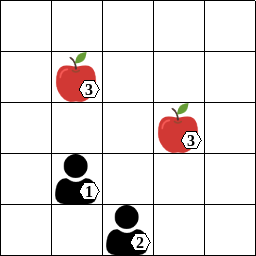
\includegraphics[width=.8\textwidth]{images/environments/lbf/lbf-5x5-2p-2f-coop.png}}
            \caption{Environment}
        \end{subfigure}
        \visible<2->{
            \begin{subfigure}[b]{.59\textwidth}
                \centering
                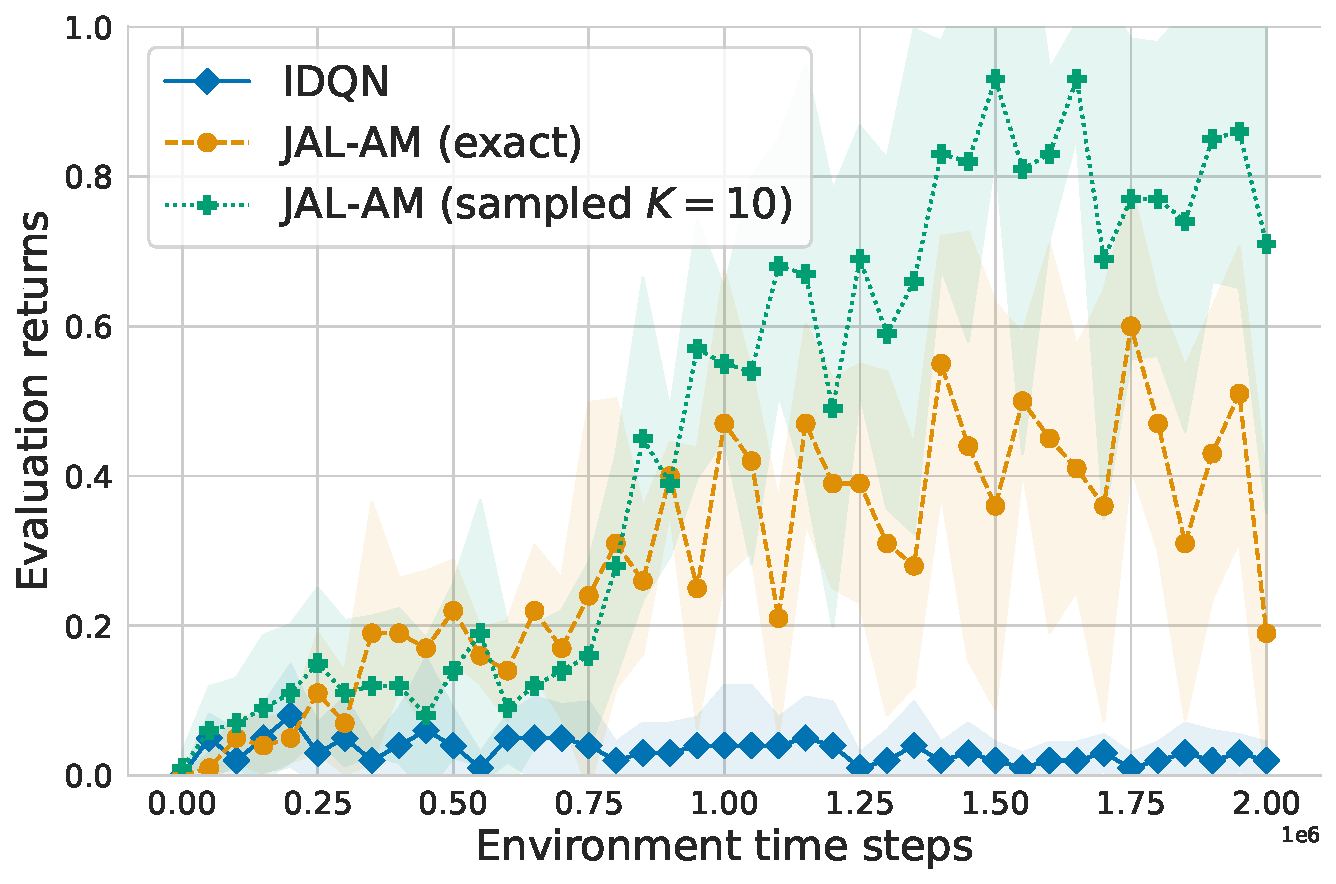
\includegraphics[width=\textwidth]{images/chapter_9/jal_am-foraging_5x5_2p_2f_coop.pdf}
                \caption{Learning curve}
            \end{subfigure}
        }
    \end{figure}
\end{frame}

\begin{frame}[t]{Learning Compact Representations of Agent Policies}
    \blist
        \item JAL-AM combines agent models and centralized value functions to compute best-response policies.
        \item Can we integrate agent models into multi-agent policy gradient algorithms, e.g.\ by conditioning policies on agent models?
    \elist

    \pause

    \begin{problembox}
        To condition policies (and value functions) of agents on the policies of other agents, we need \fat{compact} representations of the policies of other agents. How can we learn such representations?
    \end{problembox}
\end{frame}

\begin{frame}[t]{Learning Compact Representations of Agent Policies}
    \begin{figure}
        \centering
        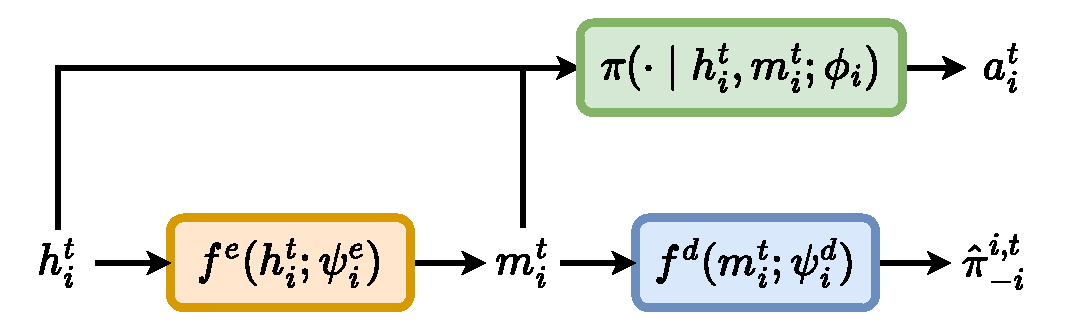
\includegraphics[width=.65\textwidth]{images/chapter_9/agent_modelling_encoder_decoder}
    \end{figure}

    Agent $i$ trains encoder-decoder architecture with
    \blist
        \item \e{Encoder $f^e$} with parameters $\psi^e_i$: given observation history $\his^t_i$ of agent $i$, output compact representation $m_i^t$ of the policies of other agents
        \item \e{Decoder $f^d$} with parameters $\psi^d_i$: given compact representation $m_i^t$, predict the policies $\hat{\pol}_{-i}^{i,t}$ of other agents
    \elist

    \pause

    \vspace{-.5em}
    
    Then, agent $i$ can condition its policy on the compact representations $m^t_i$.
\end{frame}

\begin{frame}{Learning Compact Representations of Agent Policies}
    The encoder and decoder are jointly trained to minimize the cross-entropy loss for the predicted action probabilities and true actions of all other agents:

    \bmath
        \loss(\psi_i^e, \psi_i^d) = \sum_{j\neq i} -\log \hat{\pol}_j^{i,t}(\jac_j^t) \text{\quad with \quad} \hat{\pol}_j^{i,t} = f^d\left(f^e(\his_i^t; \psi_i^e); \psi_i^d\right)_j
    \emath

    \pause

    \begin{greenbox}
        Encoder-decoder agent models can be integrated into MARL algorithm by conditioning value functions and policies on the obtained policy representations.
    \end{greenbox}
\end{frame}

\begin{frame}[t]{Compact Agent Policy Representations in LBF}
    \begin{figure}
        \centering
        \begin{subfigure}[b]{.39\textwidth}
            \centering
            \raisebox{15pt}{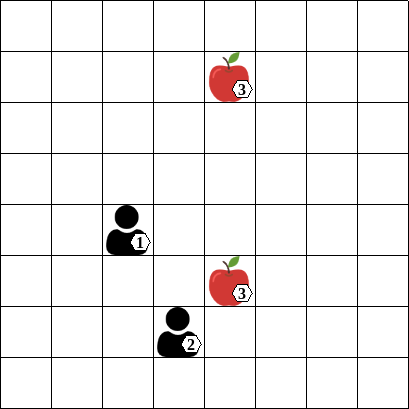
\includegraphics[width=.8\textwidth]{images/environments/lbf/lbf-8x8-2p-2f-coop.png}}
            \caption{Environment}
        \end{subfigure}
        \visible<2->{
            \begin{subfigure}[b]{.59\textwidth}
                \centering
                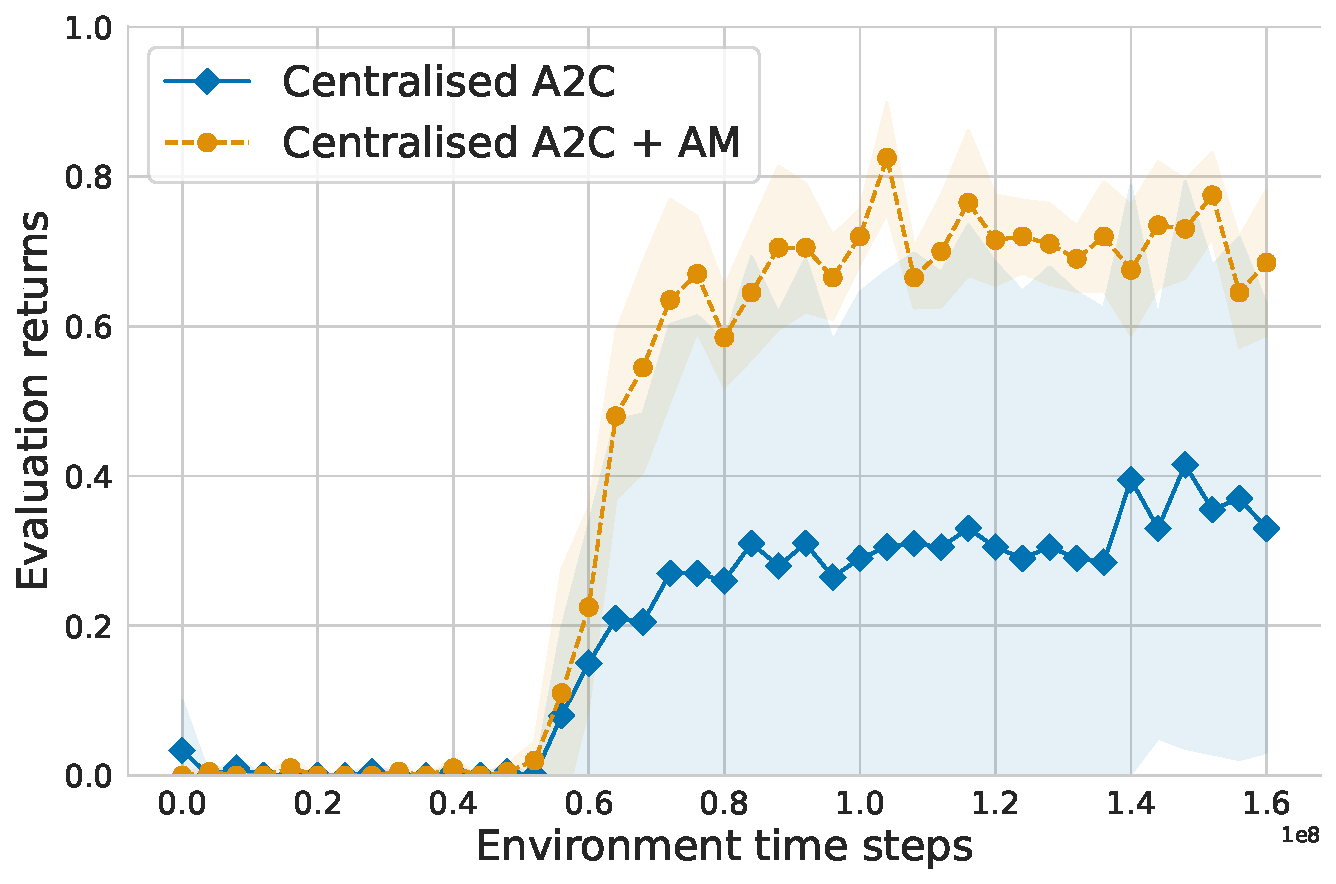
\includegraphics[width=\textwidth]{images/chapter_9/ac_am-foraging_8x8_2p_2f_coop.pdf}
                \caption{Learning curve}
            \end{subfigure}
        }
    \end{figure}
\end{frame}

\begin{frame}[t]{Reconstruction Targets to Learn Compact Representations}
    \begin{figure}
        \centering
        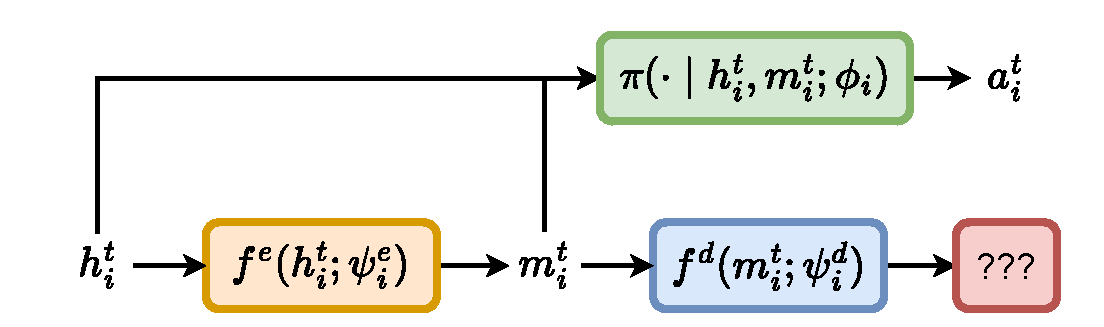
\includegraphics[width=.65\textwidth]{images/agent_modelling_encoder_decoder_targets.pdf}
    \end{figure}

    \vspace{-2em}

    \begin{notebox}
        We used the ground truth actions as information to encode by using them as targets for the decoder. We could also use
        \blist
            \item Observations -- try to capture information that other agents have access to
            \item Rewards -- try to predict the objectives that other agents optimise for
            \item \ldots
        \elist
    \end{notebox}
\end{frame}

\section{Parameter and Experience Sharing}

\begin{frame}[t]{Parameter and Experience Sharing -- Motivation}
    \begin{problembox}
        Training agents with MARL is difficult for environments with many agents due to the increased number of parameters to train $\Rightarrow$ unstable or slow training!
    \end{problembox}

    \pause

    \begin{solutionbox}
        Two approaches to improve the efficiency of training many agents:
        \blist
            \item \fat{Parameter sharing}: agents share their network parameters with each other
            \item \fat{Experience sharing}: agents share experiences with each other
        \elist
    \end{solutionbox}
\end{frame}

\begin{frame}[t]{Environments with Homogeneous Agents}
    \blist
        \item Parameter and experience sharing assume that agents are trying to learn similar or identical policies $\rightarrow$ not applicable to all environments
        \item We call agents in such environments \e{homogeneous}
        \blist
            \item<2-> \e{Strongly homogeneous agents}: All agents have the same optimal policy, i.e. $$\pol_1^* = \ldots = \pol_n^*$$
            \item<3-> \e{Weakly homogeneous agents}: Agents can be permuted and their expected returns remain the same under the permutation $\sigma: I \mapsto I$:
                \bmath
                    \exret_i(\pi)= \exret_{\sigma(i)}\left(\langle\pi_{\sigma(1)},\pi_{\sigma(2)},\dots,\pi_{\sigma(n)}\rangle\right),\ \forall i \in I 
                \emath
        \elist
    \elist
\end{frame}

\begin{frame}[t]{Environments with Homogeneous Agents -- Examples}

    \vspace{1em}

    \begin{minipage}{.49\textwidth}
        \fat{Weakly homogeneous agents:}
        \begin{figure}
            \centering
            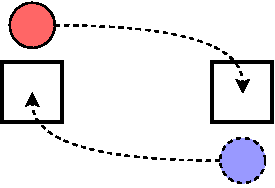
\includegraphics[height=10em]{images/chapter_9/bps_spread.pdf}
        \end{figure}

        Agents need to learn similar policies.
    \end{minipage}
    \hfill
    \begin{minipage}{.49\textwidth}
        \visible<2->{
            \fat{Strongly homogeneous agents:}
            \begin{figure}
                \centering
                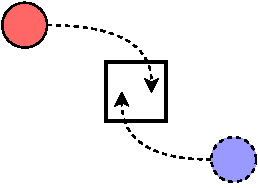
\includegraphics[height=10em]{images/chapter_9/bps_game_parametersharing.pdf}
            \end{figure}

            Agents need to learn identical policies.
        }
    \end{minipage}
\end{frame}

\begin{frame}[t]{Parameter Sharing}
    Sharing network parameters across agents is common practice to make MARL training more efficient. Share parameters across value functions, policies, or both.

    \only<1>{
        \begin{figure}
            \centering
            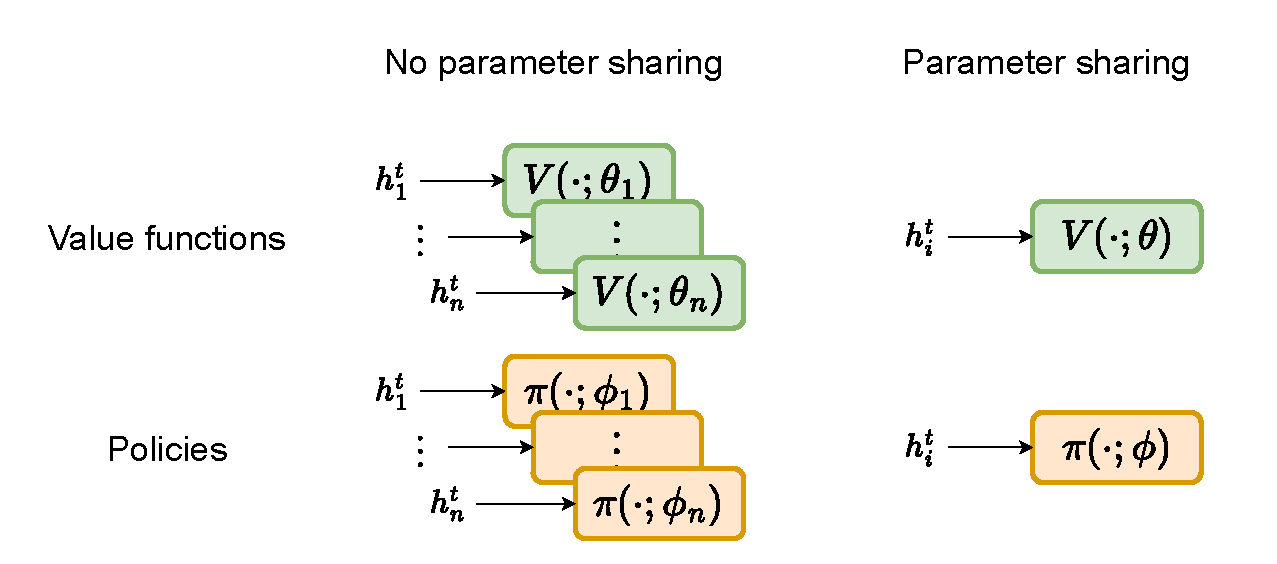
\includegraphics[height=14em]{images/parameter_sharing_mix.pdf}
        \end{figure}
    }

    \only<2->{
        \begin{minipage}{.69\textwidth}
            Parameter sharing has two primary benefits:
            \blist
                \item \fat{Scalability}: the number of parameters remains constant independent of the number of agents $\rightarrow$ less computational cost
                \item \fat{Efficiency}: shared parameters are updated using the experiences of all agents $\rightarrow$ more training data for the shared parameters
            \elist

            \pause

            The downside is that (naive) parameter sharing assumes strongly homogeneous agents.
        \end{minipage}
        \begin{minipage}{.3\textwidth}
            \begin{figure}
                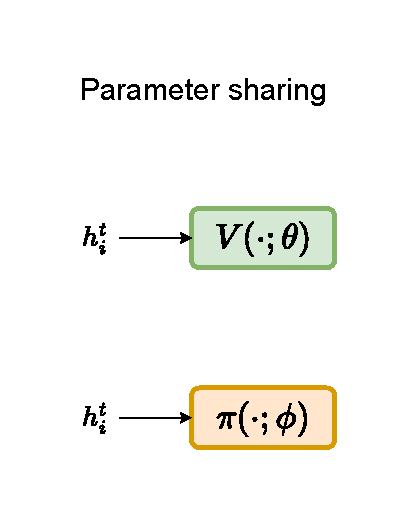
\includegraphics[height=14em]{images/parameter_sharing_cut.pdf}
            \end{figure}
        \end{minipage}

    }
\end{frame}

\begin{frame}[t]{Parameter Sharing in LBF}
    \begin{figure}
        \centering
        \begin{subfigure}[b]{.39\textwidth}
            \centering
            \raisebox{15pt}{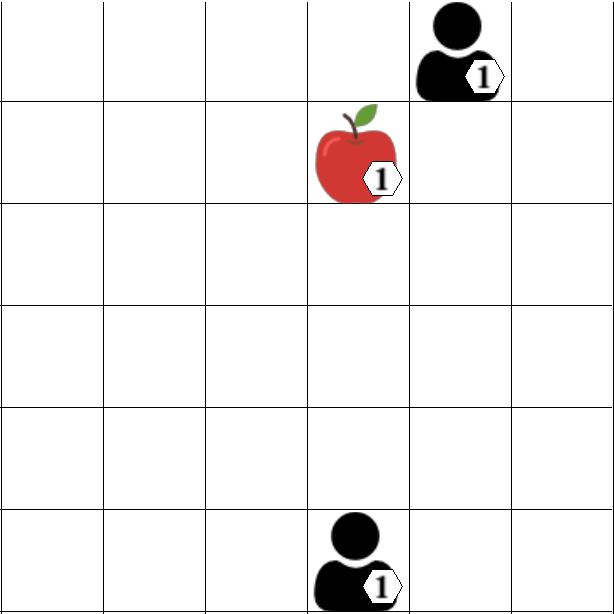
\includegraphics[width=.8\textwidth]{images/lbf_6x6-2p-1f.jpg}}
            \caption{Environment}
        \end{subfigure}
        \visible<2->{
            \begin{subfigure}[b]{.59\textwidth}
                \centering
                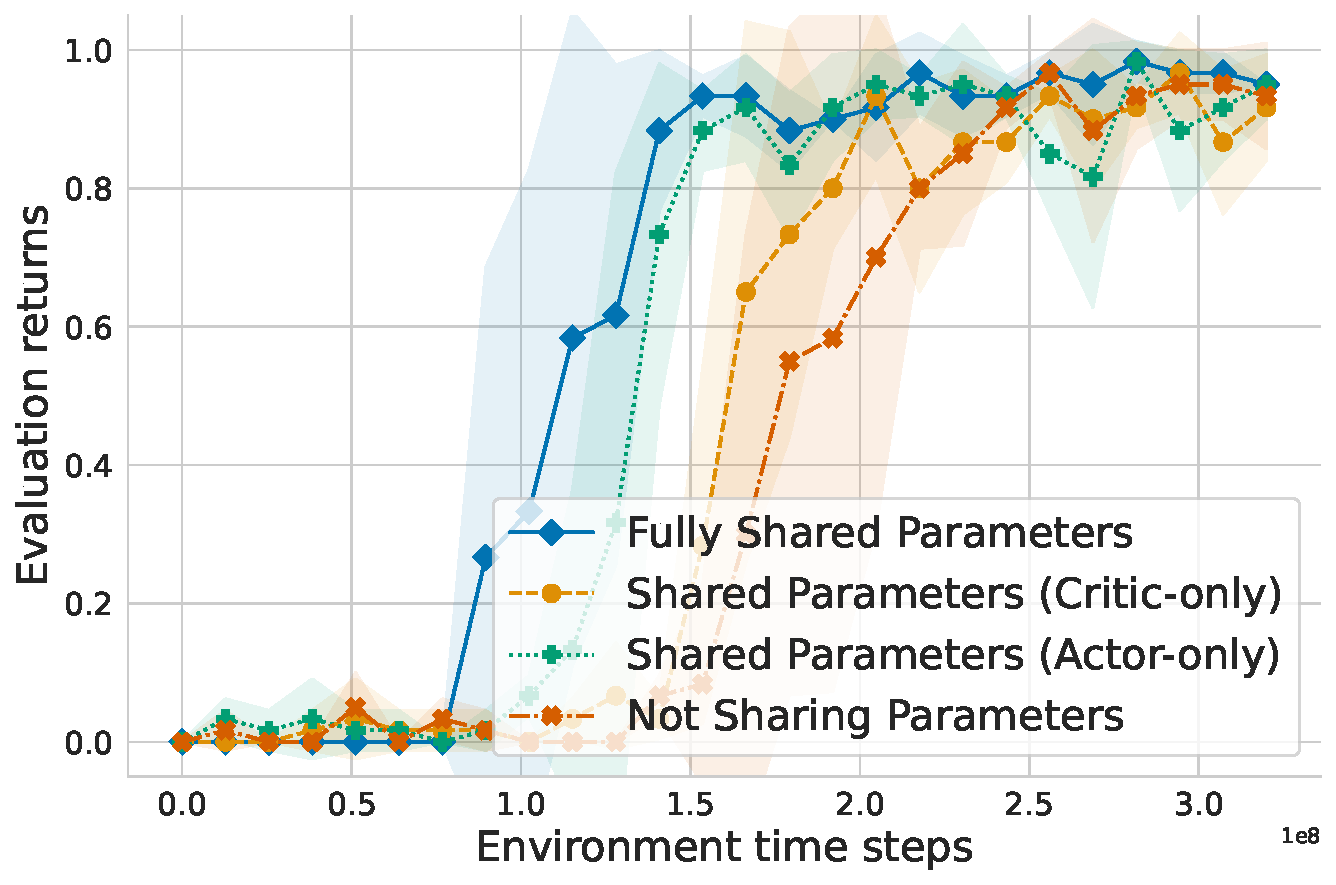
\includegraphics[width=\textwidth]{images/chapter_9/parameter-sharing.pdf}
                \caption{Learning curve}
            \end{subfigure}
        }
    \end{figure}
\end{frame}

% \begin{frame}[t]{Parameter Sharing for Weakly Homogeneous Agents}
%     So far: parameter sharing is only applicable to environments with strongly homogeneous agents.
%
%     \pause
%
%     This assumption can be relaxed to make parameter sharing applicable to environments with weakly homogeneous agents by adding agent identifiers to the inputs. For example, we can add a one-hot vector identifying agents to the input of the network to indicate for which agent the output should be computed.
%
%     \pause
%
%     However, in practice, this is often not sufficient for agents to learn meaningfully diverse/ specialised policies or value functions.
% \end{frame}

\begin{frame}{Experience Sharing for Weakly Homogeneous Agents}
    Under experience sharing, agents still learn separate policies (and value functions) but share their trajectories to allow training on the collective data.

    \pause

    \fat{Assumption}: Agents are (at least) weakly homogeneous, i.e. they need to learn similar policies.

    \pause

    \begin{notebox}
        The experiences of agent $j$ is \fat{off-policy} data for agent $i$ $\rightarrow$ experience sharing needs to use off-policy MARL algorithms or correct for the differences in data distributions.
    \end{notebox}
\end{frame}

\begin{frame}{Deep Q-Networks with Shared Experience Replay}
    We can extend IDQN with experience sharing by following the steps below:
    \blist
        \item Collect the experience of all agents in a shared replay buffer $\data_{\text{shared}}$
        \item Each agent samples from $\data_{\text{shared}}$ to update its value function
        \item Each agent optimises its value function using the typical IDQN loss
    \elist

    \pause

    \begin{notebox}
        DQN is an off-policy algorithm so it is theoretically sound to use the experience of other agents that have different policies.
    \end{notebox}
\end{frame}

\begin{frame}[t]{Shared Experience Actor-Critic (SEAC)}
    We can also extend independent actor-critic algorithms (e.g.\ IA2C and IPPO) with experience sharing by optimising the loss over the data of all agents.

    \pause
    SEAC policy loss (based on IA2C) with importance sampling (IS) weight correction:

    % \vspace{.5em}
    \bmath
        \begin{split}
            \loss(\phi_i) = & \eqnmarkbox[NavyBlue]{own}{-\left(\rew_i^t + \dsc V(\his_i^{t+1}; \theta_i) - V(\his_i^t; \theta_i)\right) \log \pol(\ac_i^t \mid \his_i^t; \phi_i)}  \\
                            &\visible<3->{- \lambda\sum_{k\neq i}\eqnmarkbox[WildStrawberry]{is}{\frac{\pi(a^t_k \mid \his^t_k; \phi_i)}{\pi(a^t_k \mid \his^t_k; \phi_k)}}\eqnmarkbox[OliveGreen]{other}{\left(\rew_k^t + \dsc V(\his_k^{t+1}; \theta_i) - V(\his_k^t; \theta_i)\right) \log \pol(\ac_k^t \mid \his_k^t; \phi_i)}}
        \end{split}
    \emath
    \annotate[yshift=1em,ultra thick]{above,left}{own}{\normalsize policy loss on own data}
    \visible<3->{
        \annotate[yshift=-.5em]{below,left}{is}{\normalsize IS correction}
        \annotate[yshift=-.5em]{below,right}{other}{\normalsize policy loss on data of agent $k$}
    }

    \pause
    \pause

    \vspace{.5em}

    Hyperparameter $\lambda$ determines weighting for the loss over the experience of other agents. The same IS weight correction can be applied to the critic loss.
\end{frame}

\section{Policy Self-Play in Zero-Sum Games}

\begin{frame}[t]{The Challenge of Zero-Sum Board Games}
    % What makes these games challenging
    Next we will take a closer look at (turn-based) zero-sum board games such as chess, shogi, or Go.

    \only<1>{
        \begin{figure}
            \centering
            \begin{subfigure}{.49\textwidth}
                \centering
                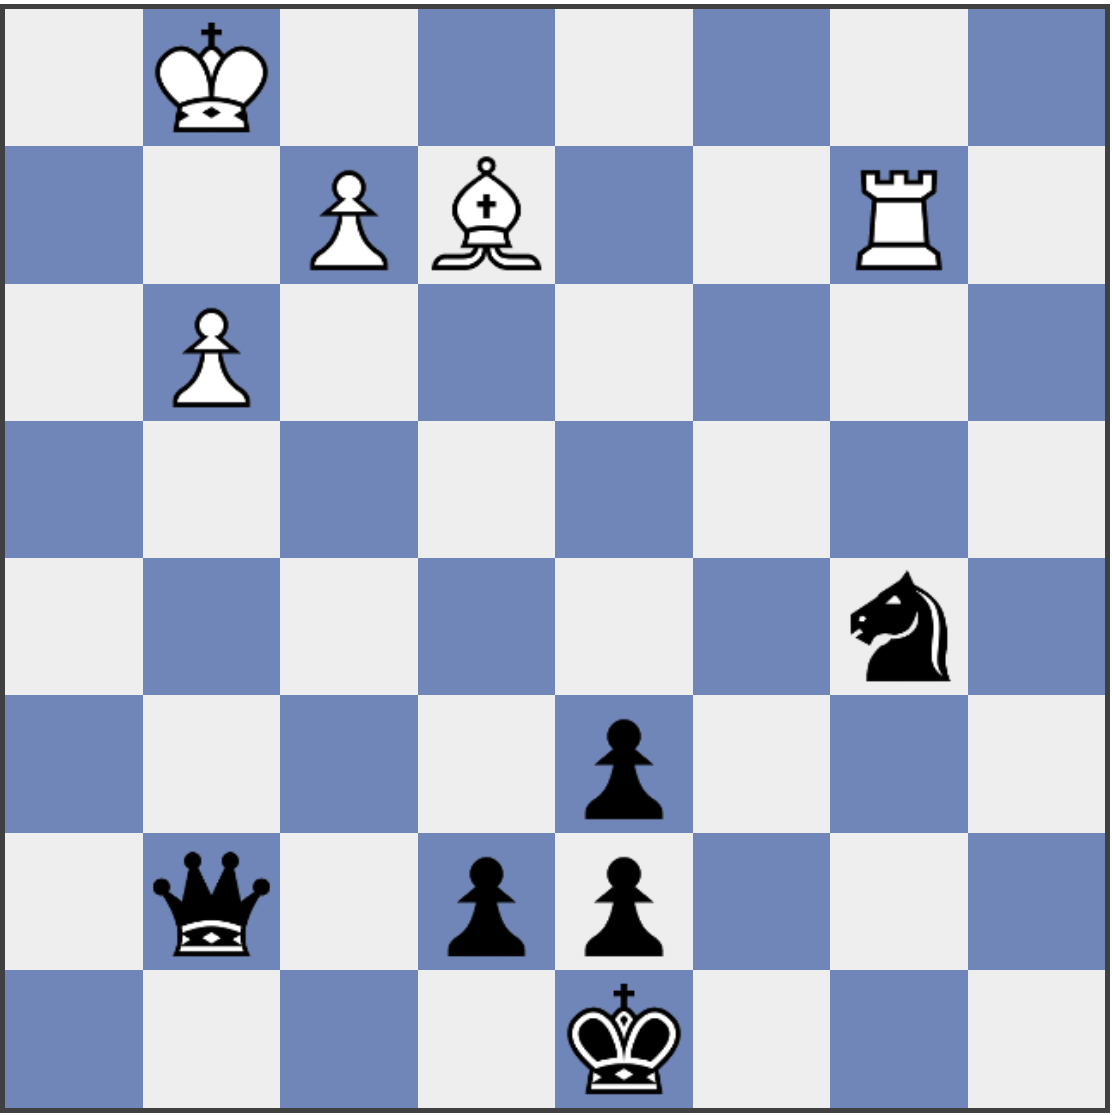
\includegraphics[width=.7\textwidth]{images/chapter_9/chess-board}
                \caption{Chess}
            \end{subfigure}
            \begin{subfigure}{.49\textwidth}
                \centering
                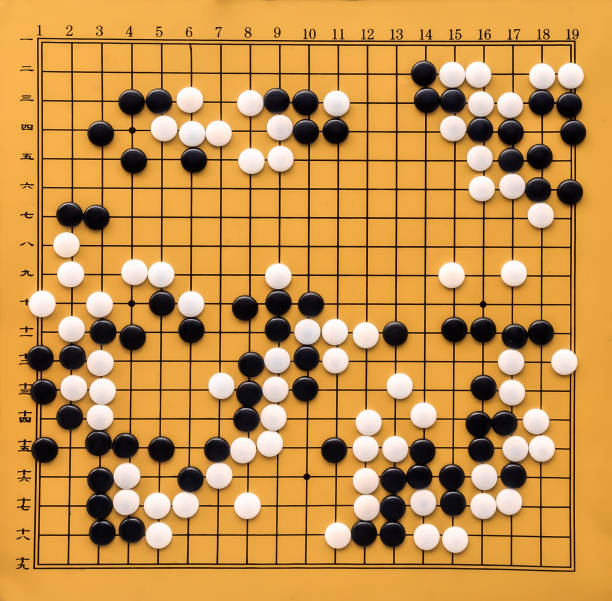
\includegraphics[width=.7\textwidth]{images/go_board}
                \caption{Go}
            \end{subfigure}
        \end{figure}
    }

    \pause

     These games are challenging decision-making problems due to
    \blist
        \item<2-> \fat{Sparse rewards:} agents only receive a reward once the game terminates (+1 for winning, -1 for losing, 0 for a draw)
        \item<3-> \fat{Large action space:} in many board games, agents can choose from a large action space (e.g. moving a particular piece to a particular position)
        \item<4-> \fat{Long horizon:} episodes can last for many time steps before reaching a terminal state
    \elist

	\visible<5->{
	    Fortunately, we can exploit the structure of these games to develop effective algorithms.}
\end{frame}

\begin{frame}[t]{Tree Search for Zero-Sum Games}
    % How to view these games as trees

    \begin{minipage}{.6\textwidth}
        \begin{figure}
            \centering
            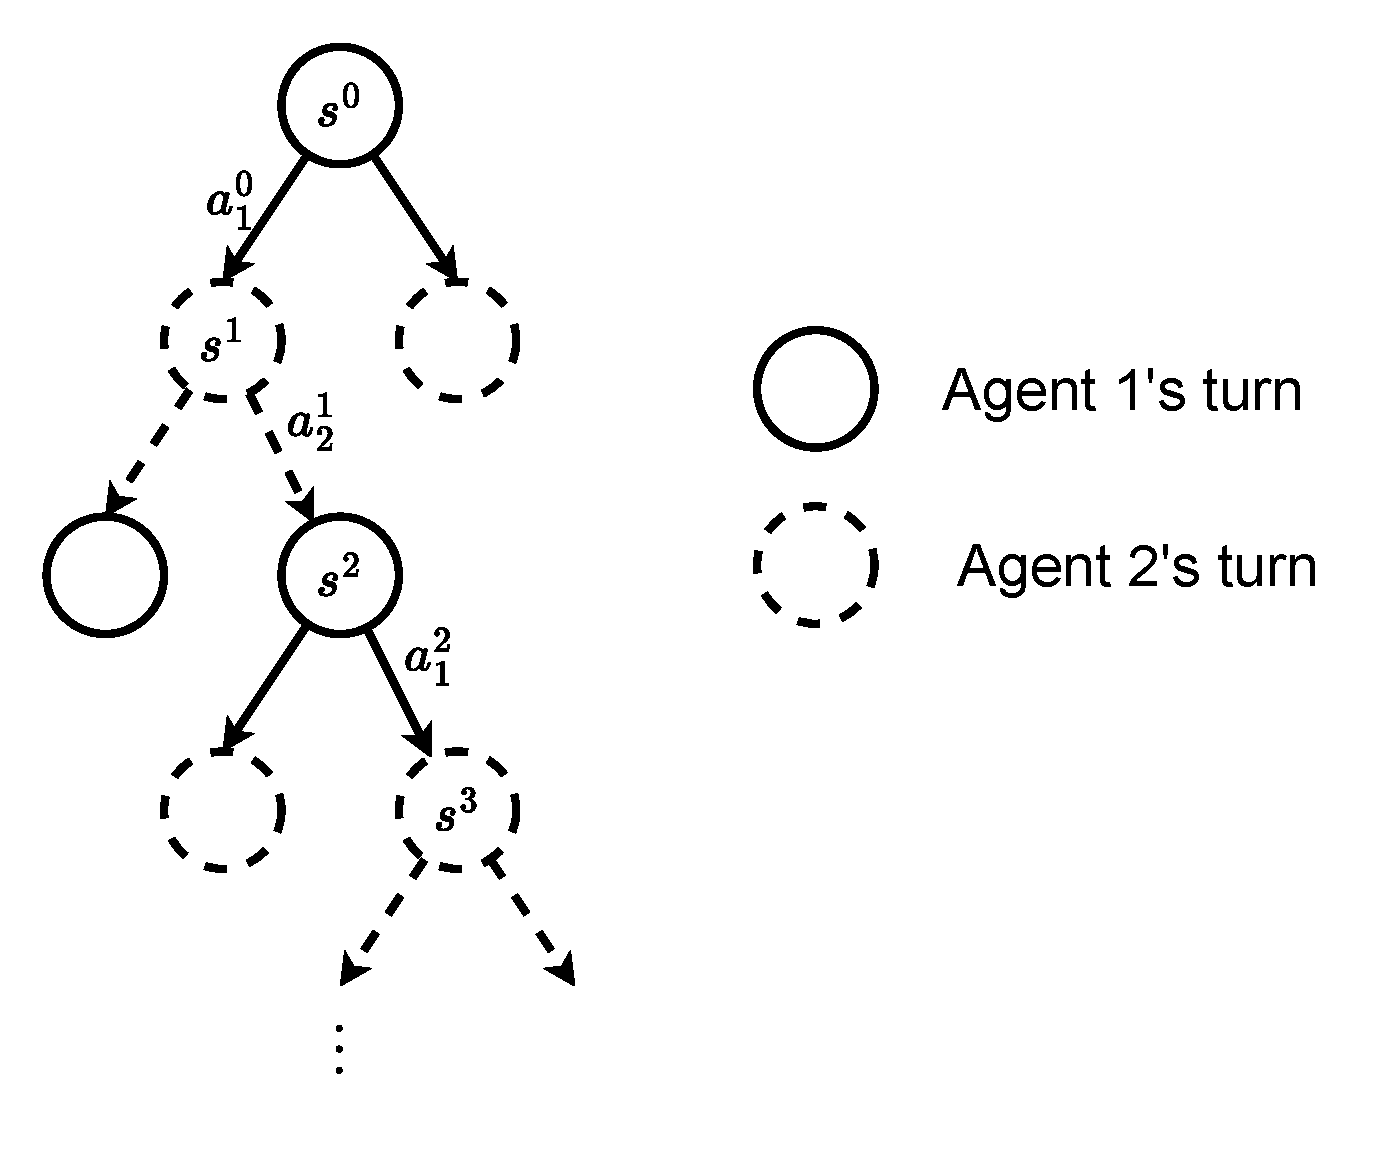
\includegraphics[width=\textwidth]{images/game-tree.pdf}
        \end{figure}
    \end{minipage}
    \hfill
    \begin{minipage}{.35\textwidth}
        \only<2>{
            We can view turn-based zero-sum games as trees where
            \blist
                \item {\it nodes} represent game states
                \item {\it edges} represent actions
                \item {\it leaves} represent terminal states
            \elist
            in each node either agent $1$ or agent $2$ makes a move.
        }
        \only<3>{
            \begin{problembox}
                The tree can grow very large depending on its
                \blist
                    \item \fat{Depth}: number of time steps until terminal states
                    \item \fat{Breadth}: number of actions available in each state
                \elist
                $\rightarrow$ makes search computationally expensive
            \end{problembox}
        }
    \end{minipage}

    % This idea is underneath many breakthroughs such as AlphaGo, AlphaZero etc.
\end{frame}

\begin{frame}[t]{Monte Carlo Tree Search (MCTS)}
    % explain MCTS  -- might be multiple slides
    \e{Monte Carlo Tree Search} (MCTS) is a tree-search algorithm that simulates (samples) possible outcomes of the game, and then updating value estimates of actions.

    \pause

    MCTS consists of three key steps that are repeated:
    \blist
        \item<3-> \fat{Simulation} simulate a game from the current state until a leaf node is reached
        \item<4-> \fat{Expansion:} expand the tree by adding a new node for the reached state if it does not exist yet
        \item<5-> \fat{Backpropagation:} update the estimated values of the nodes visited during the selection step
    \elist
\end{frame}

\begin{frame}[t]{Monte Carlo Tree Search -- Simulation}
    MCTS maintains two statistics for each visited state-action pair:
    \blist
        \item Value estimates $Q(\st, \ac)$
        \item Visitation counts $N(\st, \ac)$
    \elist

    \pause

    MCTS generates $k$ \e{simulations} from the current state by sampling actions according to a policy until a leaf node is reached. Leaf nodes are previously unvisited or terminal states.

    \pause

    To sample actions, MCTS commonly uses $\epsilon$-greedy policies with respect to action-value function $Q$, or the upper confidence bound (UCB) policy:
    \bmath
	\ach^\tau = \left\{ \begin{array}{ll}
		\ach & \text{if } N(\sth^\tau,\ach) = 0 \\[3pt]
		\arg\max_{\ach \in \Ac} \left( Q(\sth^\tau,\ach) + \sqrt{ \frac{2 \ln N(\sth^\tau)}{N(\sth^\tau,\ach)} } \right) & \text{otherwise}
		\end{array} \right.
    \emath
    that incentivises exploration of states and actions that have not been visited often.
\end{frame}

\begin{frame}[t]{Monte Carlo Tree Search -- Expansion}
    \begin{minipage}{0.39\textwidth}
        \begin{figure}
            \centering
            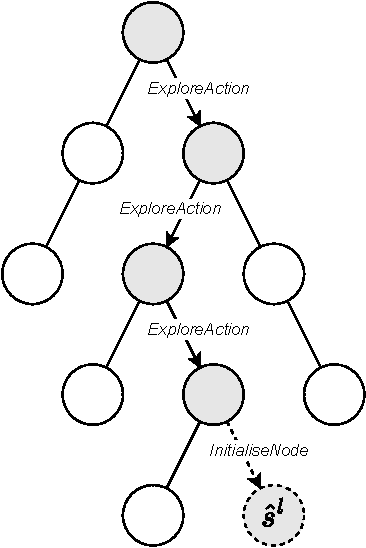
\includegraphics[width=.8\textwidth]{images/chapter_9/mcts-expand}
        \end{figure}
    \end{minipage}
    \hfill
    \begin{minipage}{0.59\textwidth}
        If leaf node is reached $\rightarrow$ \e{expand} the search tree by adding a new node for the reached state $\sth^l$\\

        \pause

        The new node is initialized with
        \blist
            \item $N(\sth^l, \ach) = 0$ for all actions $\ach$
            \item An initial value estimate $Q(\sth^l, \ach)$ for all actions $\ach$, e.g.\ from a learned value function, heuristic, or random samples of outcomes.
        \elist
    \end{minipage}
\end{frame}

\begin{frame}[t]{Monte Carlo Tree Search -- Backpropagation}
    \begin{minipage}{0.39\textwidth}
        \begin{figure}
            \centering
            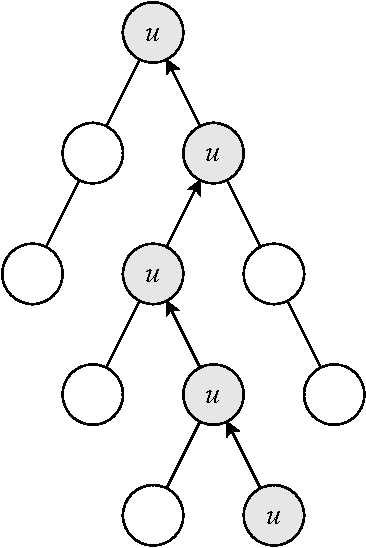
\includegraphics[width=.8\textwidth]{images/chapter_9/mcts-backprop}
        \end{figure}
    \end{minipage}
    \hfill
    \begin{minipage}{0.59\textwidth}
        Once a value estimate $\ret$ for the leaf node is obtained $\rightarrow$ \e{backpropagate} rewards and value estimates starting from the leaf node up to the root node.\\

        \pause

        For each visited state-action pair $(\sth^\tau, \ach^\tau)$, we increment the visitation count and update the value:
        \bmath
            Q(\sth^\tau,\ach^\tau) \gets Q(\sth^\tau,\ach^\tau) + \frac{1}{N(\sth^\tau,\ach^\tau)} \left[ \ret - Q(\sth^\tau,\ach^\tau) \right]
        \emath

        \pause

        (Any RL TD update rule can be used to update the value estimates.)
    \end{minipage}
\end{frame}

\begin{frame}[t]{Monte Carlo Tree Search -- Action Selection}
    Simulation, expansion, and backpropagation steps are repeated at every time step to iteratively grow the search tree and obtain better value estimates.\\ \ \\

    \pause

    Following $k$ simulations form the current state $\st^t$, the best action is selected. This process can be done by choosing the action with:
    \blist
        \item highest value estimate: $BestAction(\st^t) = \arg\max_{\ach \in \Ac} Q(\st^t, \ach)$
        \item highest visitation count: $BestAction(\st^t) = \arg\max_{\ach \in \Ac} N(\st^t, \ach)$
    \elist

\end{frame}

\begin{frame}[t]{Monte Carlo Tree Search -- Pseudocode}
    \scalebox{0.65}{
        \begin{minipage}{0.95\linewidth}
            \vspace{-1em}

            \balg{Monte Carlo tree search (MCTS) for MDPs}{mcts}
                \State Repeat for every episode:
                \For{$t = 0,1,2,3,...$} \label{alg:mcts-time}
                        \State Observe current state $\st^t$ \label{alg:mcts-st}
                        \For{$k$ simulations}
                                \State $\tau \gets t$
                                \State $\sth^\tau \gets \st^t$ \Comment{Perform simulation}
                                \While{$\sth^\tau$ is non-terminal and $\sth^\tau$-node exists in tree}
                                        \State $\ach^\tau \gets ExploreAction(\sth^\tau)$ \label{alg:mcts-explore}
                                        \State $\sth^{\tau+1} \sim \Stf(\cdot \mid \sth^\tau, \ach^\tau )$
                                        \State $\rewh^\tau \gets \Rew(\sth^\tau,\ach^\tau,\sth^{\tau+1})$
                                        \State $\tau \gets \tau + 1$
                                \EndWhile
                                \If{$\sth^\tau$-node does not exist in tree}
                                        \State $InitializeNode(\sth^\tau)$ \Comment{Expand tree} \label{alg:mcts-init}
                                \EndIf
                                \While{$\tau > t$} \Comment{Backpropagate}
                                        \State $\tau \gets \tau - 1$
                                        \State $Update(Q,\sth^\tau,\ach^\tau)$ \label{alg:mcts-update}
                                \EndWhile
                        \EndFor
                        \State Select action $\ac^t$ for state $\st^t$:
                        \State \quad $\pol^t \gets BestAction(\st^t)$ \label{alg:mcts-bestact}
                        \State \quad $\ac^t \sim \pol^t$
                \EndFor
            \ealg
        \end{minipage}
    }
    \hfill
    \begin{minipage}{0.35\textwidth}
        \pause
        \begin{notebox}
            MCTS assumes known transition function $\Stf$ and reward function $\Rew$.\\

            \pause

            Can learn estimates of these functions from data to simulate possible outcomes of the game.
        \end{notebox}
    \end{minipage}
\end{frame}

\begin{frame}[t]{Self-Play Monte Carlo Tree Search}
    In zero-sum games with symmetrical roles and egocentric observations, agents can use the same policy to control both players \pause $\rightarrow$ learn a policy in \e{self-play}

    \begin{figure}[t]
	\centering
	\begin{subfigure}[b]{0.35\textwidth}
            \centering
            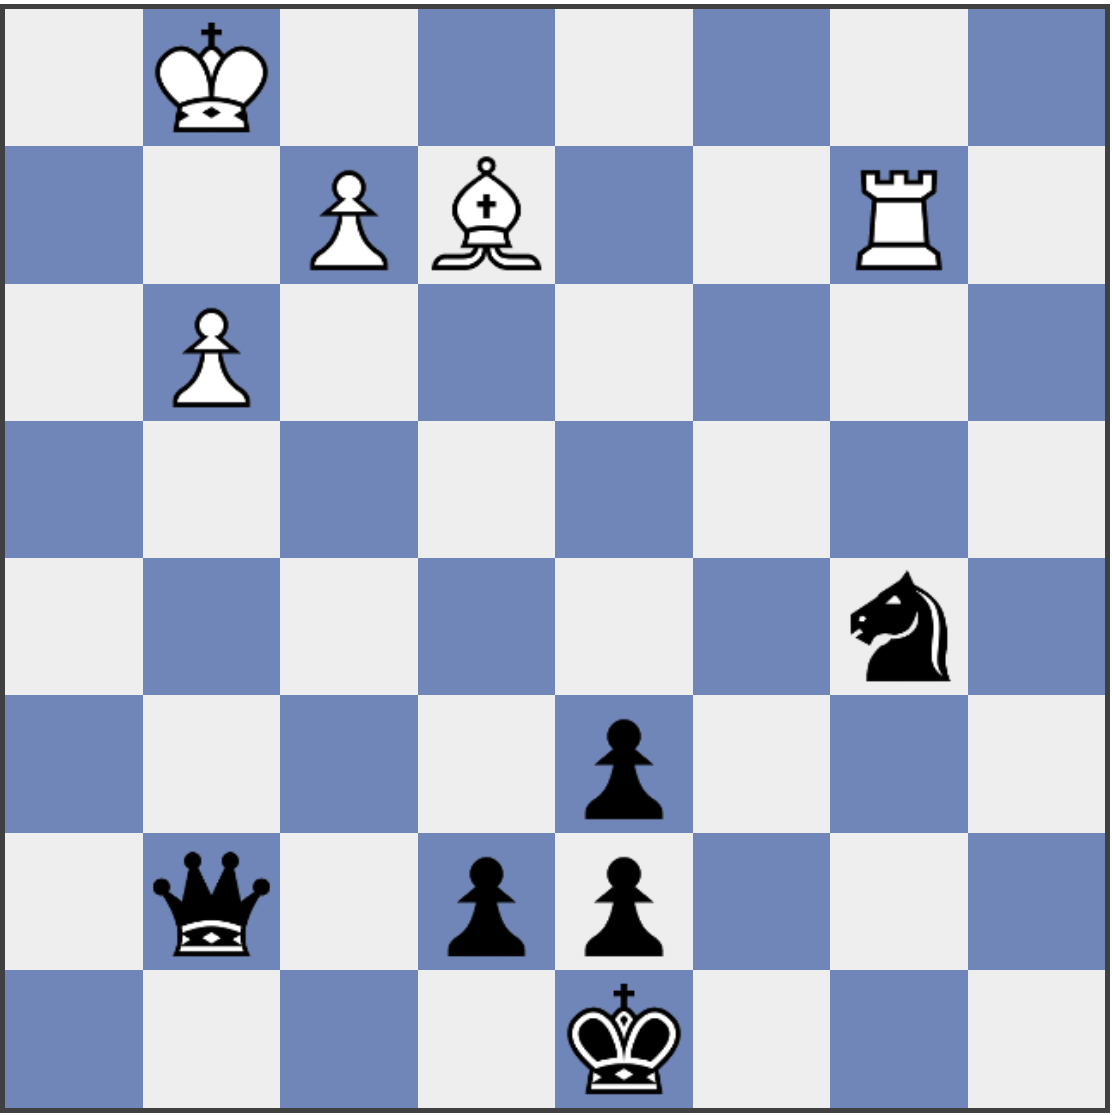
\includegraphics[width=.9\textwidth]{images/chapter_9/chess-board}
            \caption{Agent 1 perspective}
	\end{subfigure}
	\hspace{5em}
	\begin{subfigure}[b]{0.35\textwidth}
            \centering
            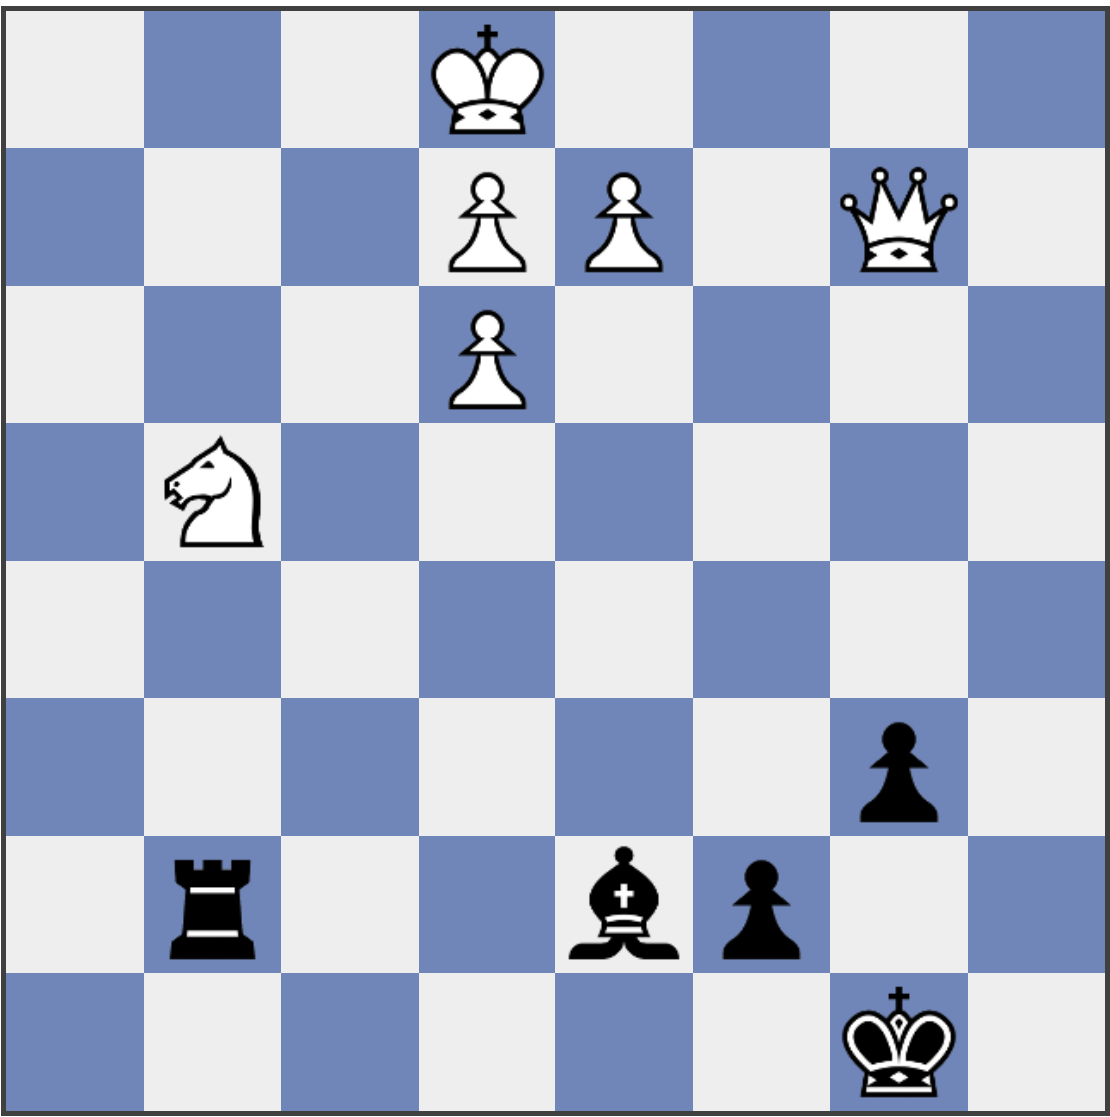
\includegraphics[width=.9\textwidth]{images/chapter_9/chess-board-transform}
            \caption{Agent 2 perspective}
	\end{subfigure}
    \end{figure}

\end{frame}

\begin{frame}[t]{AlphaZero -- Self-Play MCTS with Deep Learning}
    \e{AlphaZero}: combine self-play MCTS with deep learning to learn value estimates and policies $\rightarrow$ reached superhuman performance in Go, chess, and shogi!

    \vspace{.5em}

    \begin{minipage}{.69\textwidth}
        \visible<2->{
            Learn functions with parameters $\theta$ conditioned on state $\st$:
            \blist
                \item Value estimate $V(\st; \theta)$
                \item Policy $\pol(\cdot \mid \st; \theta)$
            \elist
        }

        \visible<3->{
            For each episode, a triplet $(\st, \pol, z)$ of data is stored where
            \blist
                \item $\st$ are the states
                \item $\pol$ are policy distributions computed by $BestAction$
                \item $z$ is the game outcome (+1 for win, -1 for loss, 0 for draw)
            \elist
        }
    \end{minipage}
    \hfill
    \begin{minipage}{.29\textwidth}
        \begin{figure}
            \centering
            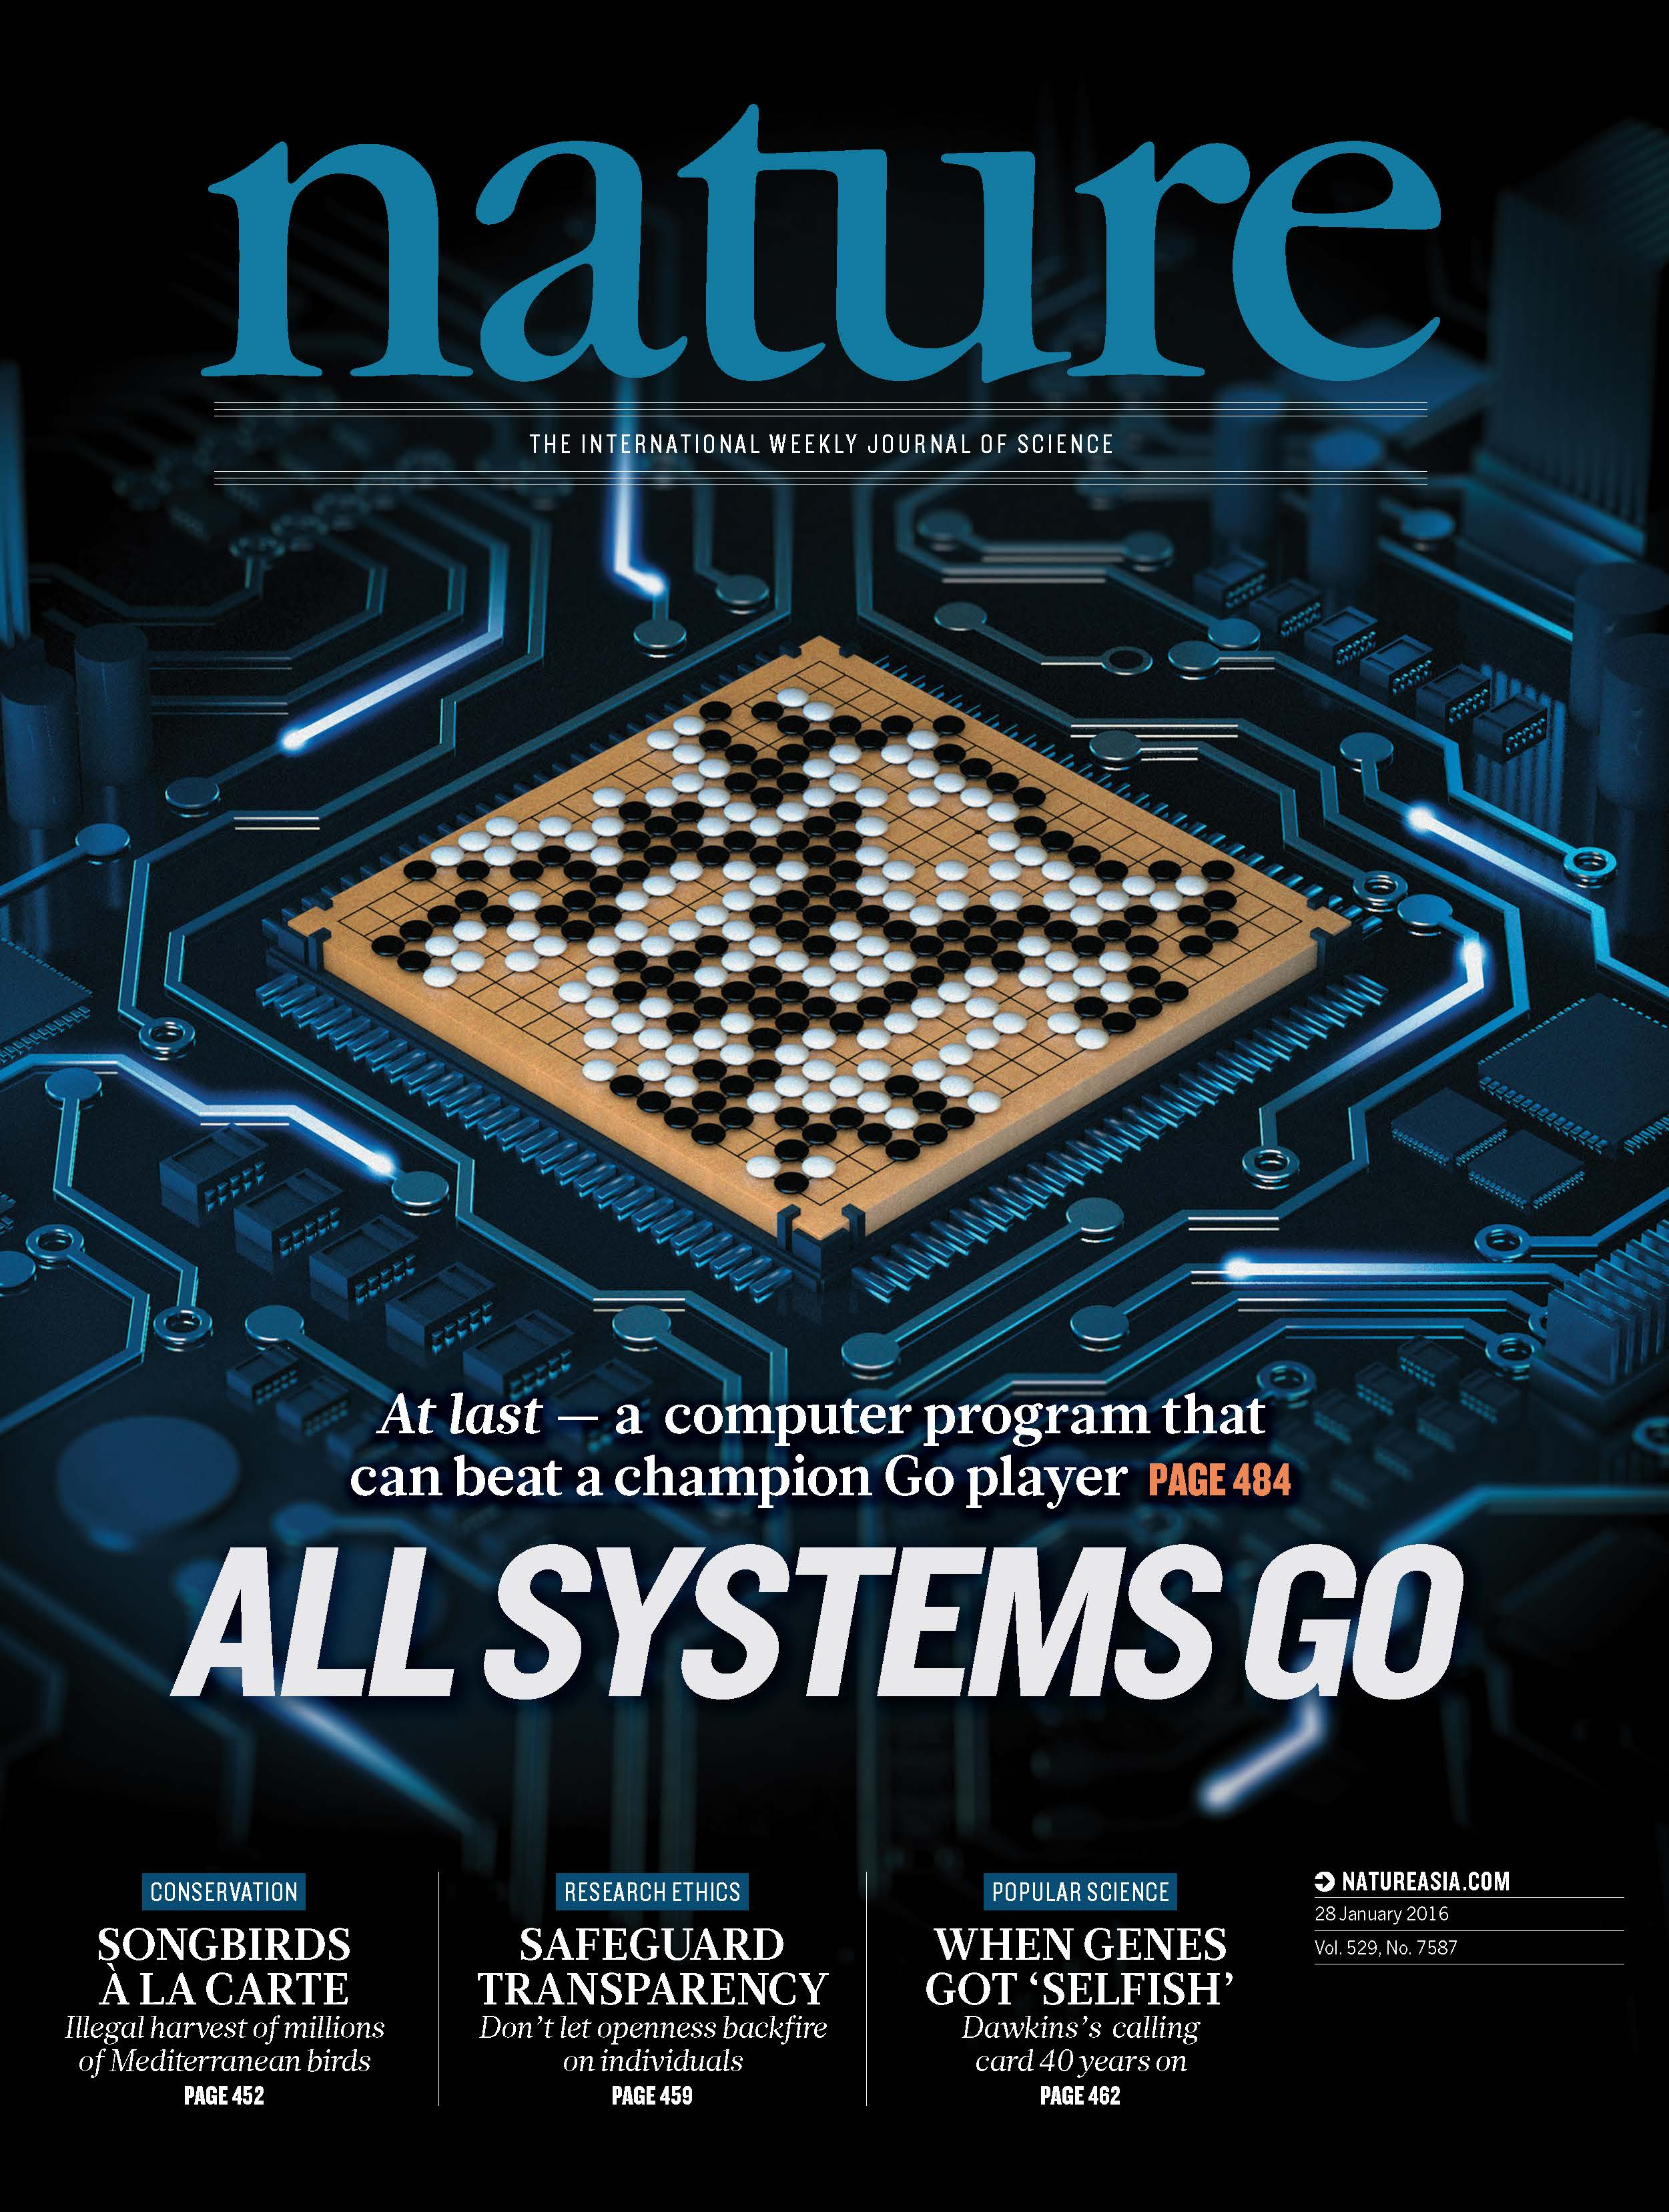
\includegraphics[width=\textwidth]{images/nature_alphago}
        \end{figure}
    \end{minipage}
\end{frame}

\begin{frame}[t]{AlphaZero -- Self-Play MCTS with Deep Learning}
    The network is randomly initialized and trained using sampled batches of data to minimise the following combined loss:
    \vspace{-.5em}
    \begin{align*}
        \loss(\theta) &= \loss_{\text{value}} + \loss_{\text{policy}} + c\, || \theta ||^2\\
        \loss_{\text{value}} &= \ex{(\st, \pol, z) \sim \data}{\left(V(\st; \theta) - \ret\right)^2} \\
        \loss_{\text{policy}} &= \ex{(\st, \pol, z) \sim \data}{\pol^\top \log \pol(\cdot \mid \st; \theta)} \\
    \end{align*}

    \pause
    \vspace{-2em}
    For exploration, AlphaZero combines a UCB policy with the learned policy:
    \vspace{-.5em}
    \bmath
	\ach^\tau = \left\{ \begin{array}{ll}
		\ach & \text{if } N(\sth^\tau,\ach) = 0 \\[3pt]
		\arg\max_{\ach \in \Ac} \left( Q(\sth^\tau,\ach) + C(\sth^\tau) P(\sth^\tau,\ach)\frac{ \sqrt{ N(\sth^\tau) } }{ 1 + N(\sth^\tau,\ach) } \right) & \text{otherwise}
		\end{array} \right.
    \emath

    \vspace{-1em}
    with the additional exploration rate $C(\sth^\tau)$.
\end{frame}

% \begin{frame}[t]{AlphaZero: Self-Play MCTS with Deep Learning -- Performance}
%     AlphaZero outperformed previously known superhuman algorithms in chess, shogi, and Go:
%     \begin{figure}
% 	\centering
% 	\begin{tabular}{lccc}
%             \toprule
%             AlphaZero (playing white) vs. & Win & Draw & Loss \\
%             \midrule
%             Stockfish (chess) & 29.0\% & 70.6\% & 0.4\% \\
%             Elmo (shogi) & 84.2\% & 2.2\% & 13.6\% \\
%             AlphaGo Zero (Go) & 68.9\% & -- & 31.1\% \\
%             \bottomrule
% 	\end{tabular}
%     \end{figure}
% \end{frame}

\section{Population-Based Training}

\begin{frame}[t]{Population-Based Training -- Self-Play for General-Sum Games}
    % Motivation of extending self-play ideas to general-sum games
    \begin{problembox}
        With MCTS, we focused on policy self-play in \fat{two-agent zero-sum} games. Can we extend the idea of self-play to \fat{general-sum} games with \fat{more than two agents}?
    \end{problembox}

    \pause
    \vspace{1em}

    \e{Population-based training} is a generalisation of self-play to general-sum games:
    \blist
        \item Maintain a \fat{population of policies} representing possible strategies of the agent
        \item Evolve populations so they become more effective against the populations of other agents
        \item We denote the population of policies for agent $i$ at generation $k$ as $\Pol_i^k$.
    \elist
\end{frame}

\begin{frame}{Population-Based Training -- Overview}
    First, initialize a population of policies for each agent (e.g.\ random policies).
    
    \vspace{10pt}

    For each generation, population-based training then follows two steps:
    \blist
        \item<2-> \fat{Evaluation:} evaluate the performance of the policies in the population by playing games against policies of the current populations of all other agents
        
        \item<3-> \fat{Evolution:} based on evaluation results, evolve the populations of all agents. This can be done by selecting a subset of high-performing policies, mutating existing policies, or adding new policies to the population.
    \elist
    
    \visible<4->{
    This process is repeated until convergence or for a fixed number of generations.}
\end{frame}

\begin{frame}[t]{Policy Space Response Oracles (PSRO)}
    \e{Policy space response oracles} (PSRO) is a population-based MARL algorithm with the following steps:

    \vspace{1em}

    \begin{columns}
        \begin{column}{0.65\textwidth}
            \begin{enumerate}
                \item<2-> Initialize populations of random policies for each agent
                \item<3-> Construct a \fat{meta-game} $M^k$ at generation $k$ from the populations of all agents as a (non-repeated) normal-form game with
                    \blist
                        \item Actions: policies of agent populations, i.e.\ $\Ac_i = \Pol_i^k$
                        \item Rewards: returns of joint policies $\langle \pol_1, \ldots, \pol_n \rangle$, i.e.\ $\Rew_i(\pol_1, \ldots, \pol_n) = \exret_i(\pol_1, \ldots, \pol_n)$.
                    \elist
            \end{enumerate}
        \end{column}
        \begin{column}{0.3\textwidth}
            \visible<3->{
                \begin{figure}
                    \centering
                    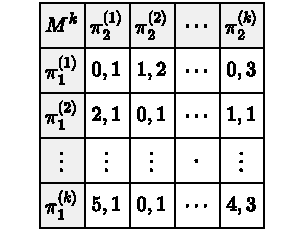
\includegraphics[width=.95\textwidth]{images/chapter_9/psro-game}
                \end{figure}
            }
        \end{column}
    \end{columns}

\end{frame}

\begin{frame}[t]{Policy Space Response Oracles -- Construct Meta-Game}
    \begin{minipage}{0.35\textwidth}
        \vspace{2em}
        \begin{figure}
            \centering
            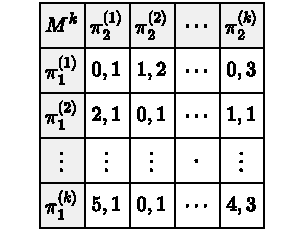
\includegraphics[width=.9\textwidth]{images/chapter_9/psro-game}
        \end{figure}
    \end{minipage}
    \hfill
    \begin{minipage}{0.6\textwidth}
        \begin{problembox}
             Need to compute the expected returns of each agent for any joint policy $\langle \pol_1, \ldots, \pol_n \rangle$ in the meta-game. How can we do this?
        \end{problembox}

        \pause
        \begin{solutionbox}
            Compute average returns of each agent over multiple episodes of the underlying game with respective joint policy $\rightarrow$ converges to expected returns in the limit.
        \end{solutionbox}
    \end{minipage}
\end{frame}

\begin{frame}[t]{Policy Space Response Oracles -- Solve Meta-Game}
    \vspace{.5em}

    \begin{minipage}{0.39\textwidth}
        \begin{figure}
            \centering
            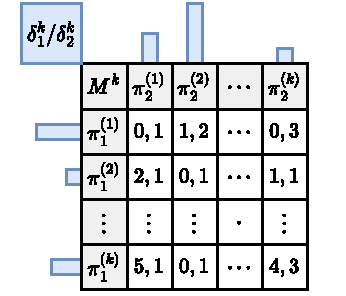
\includegraphics[width=\textwidth]{images/chapter_9/psro-solve}
        \end{figure}
    \end{minipage}
    \hfill
    \begin{minipage}{0.54\textwidth}
        Compute a \fat{solution to the meta-game} $M^k$ following some solution concept, e.g.\ a Nash equilibrium.\\

        \pause

        Solution to the meta-game: distributions $\delta_i^k$ over policies in the population of agent $i$ (for each agent $i\in\Ag$).

        % \pause
        % \begin{notebox}
        %     To avoid overfitting to few policies, we can encourage diversity by enforcing that $\delta_i^k(\pol_i) > \epsilon$ for each policy $\pol_i \in \Pol_i^k$ of agent $i$ for some small $\epsilon > 0$.
        % \end{notebox}
    \end{minipage}
\end{frame}

\begin{frame}[t]{Policy Space Response Oracles -- Add Best-Response Policies}
    \begin{minipage}{0.39\textwidth}
        \vspace{1.5em}
        \begin{figure}
            \centering
            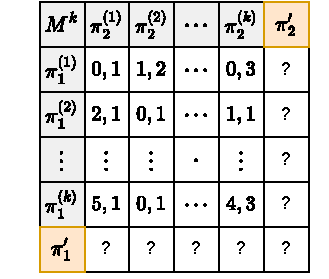
\includegraphics[width=.95\textwidth]{images/chapter_9/psro-oracle}
        \end{figure}
    \end{minipage}
    \hfill
    \begin{minipage}{0.59\textwidth}
        Each agent $i$ determines an effective \fat{oracle policy} $\pol'_i$ against the solution distribution of the other agents and adds this policy to its population:
        \bmath
            \Pol_i^{k+1} = \Pol_i^k \cup \{ \pol'_i \}
        \emath

        \pause

        For example, agent $i$ might determine its best-response policy
        \bmath
            \pol'_i \in \argmax_{\pol_i} \ex{\pol_{-i} \sim \delta_{-i}^k}{ \exret_i( \con{ \pol_i , \pol_{-i} } ) }
        \emath
        by training a policy $\pol'_i$ using RL against sampled policies of the other agents.
    \end{minipage}
\end{frame}


\begin{frame}[t]{Policy Space Response Oracles -- Pseudocode}
    % Explain over multiple slides / skip or only mention final idea of convergence
    \balg{Policy space response oracles (PSRO)}{psro}
        \State Initialize populations $\Pol_i^1$ for all $i \in \Ag$ (e.g.,\ random policies)
        \For{each generation $k = 1,2,3,...$}
                \State Construct meta-game $M^k$ from current populations $\{ \Pol_i^k \}_{i \in \Ag}$
                \State Use meta-solver on $M^k$ to obtain distributions $\{ \delta_i^k \}_{i \in \Ag}$
                \For{each agent $i \in \Ag$} \Comment{Train best-response policies} \label{alg:psro-br-loop}
                        \For{each episode $e = 1,2,3,...$}
                                \State Sample policies for other agents $\pol_{-i} \sim \delta_{-i}^k$
                                \State Use \sa\rl to train $\pol'_i$ wrt. $\pol_{-i}$ in underlying game $G$
                        \EndFor
                        \State Grow population $\Pol_i^{k+1} \gets \Pol_i^k \cup \{ \pol'_i \}$
                \EndFor
        \EndFor
    \ealg

    \vspace{-1em}

    \pause
    Repeat this process until policy populations converge (new best-response policies are already in the respective populations), or for a fixed number of generations.
\end{frame}

\begin{frame}[t]{Policy Space Response Oracles in Rock-Paper-Scissors}
    If PSRO computes exact Nash equilibria solutions to the meta-game, and computes exact best-response policies, then the population distributions of PSRO converge to the Nash equilibrium of the underlying game.

    \pause

    For example for rock-paper-scissors for two agents, with initial populations deterministically choosing rock and paper, respectively:
    \begin{figure}[t]
	\centering
	\setstretch{1.2}
	\begin{tabular}{ p{1em} c c c c c c }
		\toprule
		$k$ & $\Pol_1^k$ & $\Pol_2^k$ & $\delta_1^k$ & $\delta_2^k$ & $\pol'_1$ & $\pol'_2$ \\
		\midrule
		1 & \ul{R} & \ul{P} & $1$ & $1$ & S & P \\
		2 & R,\ul{S} & P & $(0,1)$ & $1$ & S & R \\
		3 & R,S & \ul{R},P & $(\frac{2}{3},\frac{1}{3})$ & $(\frac{2}{3},\frac{1}{3})$ & P & R/P \\
		4 & R,\ul{P},S & R,P & $(0,\frac{2}{3},\frac{1}{3})$ & $(\frac{1}{3},\frac{2}{3})$ & R & S \\
		5 & R,P,S & R,P,\ul{S} & $(\frac{1}{3},\frac{1}{3},\frac{1}{3})$ & $(\frac{1}{3},\frac{1}{3},\frac{1}{3})$ & R/P/S & R/P/S \\
		\bottomrule
	\end{tabular}
    \end{figure}
\end{frame}

\begin{frame}{AlphaStar -- GrandMaster in StarCraft II}
    StarCraft II is a real-time strategy game for two or more players in which players have to collect resources, build infrastructure and armies to defeat their opponents.

    \only<1>{
        \begin{figure}
            \centering
            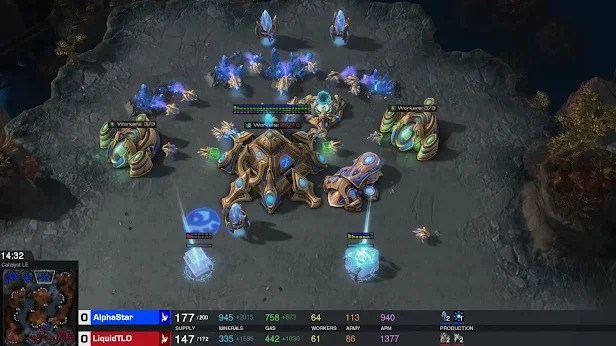
\includegraphics[width=.6\textwidth]{images/alphastar_starcraft}
            \caption{StarCraft II game, image source: \url{https://deepmind.google/discover/blog/alphastar-mastering-the-real-time-strategy-game-starcraft-ii/}.}
        \end{figure}
    }

    \pause

    StarCraft II is challenging due to
    \blist
        \item<2-> \fat{Sparse rewards:} players only receive a terminal reward at the end of the game
        \item<2-> \fat{Large action space:} players choose between many actions constituting of a type (e.g., build, move, attack), which unit should execute the action, and the target of the action
        \item<2-> \fat{Long horizon:} games can last for thousands of time steps
        \item<3-> \fat{Partial observability:} players only observe a limited view of the game state
        \item<3-> \fat{Diversity of strategies:} players choose between three available races offering many units and possible strategies
    \elist
\end{frame}

\begin{frame}[t]{AlphaStar -- GrandMaster in StarCraft II}
    \e{AlphaStar} pre-trains policies for each race using supervised imitation learning on human demonstrations from observation histories and game statistics.

    \pause

    After pre-training, AlphaStar trains its policies with deep RL using a population-based training approach called \fat{league training}: for each race, maintain a league with three types of populations, each with a different objective:
    \blist
        \item<3-> \fat{Main agents}: largely trained in self-play and against any prior policy
        \item<4-> \fat{Exploiter agents}: largely trained against the current main agents to learn to exploit their weaknesses
        \item<5-> \fat{League exploiter agents}: trained against all agents in the league to identify effective strategies missing in the league
    \elist

    \pause
    \pause
    \pause
    \pause

    \vspace{-.5em}
    Agents of each type are added to the league whenever they become effective (measured by win rates) against their respective opponents.
\end{frame}

\begin{frame}[t]{AlphaStar -- GrandMaster in StarCraft II}
    During population-based training, AlphaStar computes distributions over the policies in the league to train any policy $\pol'_i$ against using \e{prioritized fictitious self-play} (PFSP):
    \bmath
	\delta_i^k(\pol_i) \, \propto \ f\left( \pr [\pol'_i \text{ wins against } \pol_i] \right)
    \emath
    which is proportional to the probability of the agent winning against the policy $\pol_i$.

    \pause

    and $f : [0,1] \to [0,\infty)$ is a weighting function with two components:
    \blist
	\item $f_{hard}$: focus on the most difficult opponent policies for $\pol'_i$
	\item $f_{var}$ focus on opponent policies that are at a similar level of performance as $\pol'_i$
    \elist

    \pause

    Win probabilities are estimated by running multiple matches of $\pol'_i$ versus $\pol_i$.

    \pause

    $\rightarrow$ reached ``GrandMaster'' level in StarCraft II (top 0.2\% of ranked human players).
\end{frame}

\begin{frame}{Summary}
    \fat{We covered:}
        \blist
            \item Agent modelling with deep learning
            \item Parameter and experience sharing
            \item Policy self-play in zero-sum games
            \item Population-based training
        \elist

    % \fat{Next we'll cover:}
    %     \blist
    %         \item TODO
    %     \elist
        
\end{frame}

\end{document}
